\documentclass[10pt]{memoir}
\setstocksize{220mm}{155mm} 	        
\settrimmedsize{220mm}{155mm}{*}	
\settypeblocksize{170mm}{116mm}{*}	
\setlrmargins{18mm}{*}{*}
\setulmargins{*}{*}{1.2}
%\setlength{\headheight}{5pt}%
\checkandfixthelayout[lines]
\linespread{1.16}
\flushbottom

%%% Hyphenation settings
\usepackage[htt]{hyphenat}
\hyphenation{he-lio-trope opos-sum}
\tracingparagraphs=1
%Hyphenation in Devanāgarī of the edition still missing? Probably this needs to be modified in babel-iast package? 

%%% babel
\usepackage[english]{babel}
\usepackage{babel-iast/babel-iast}

\babelfont[iast]{rm}[Renderer=Harfbuzz, Scale=1.3]{AdishilaSan}%AdishilaSan}
\babelfont[english]{rm}{Adobe Text Pro}

%%% more functionality
\PassOptionsToPackage{hyphens}{url}
\usepackage{hyperref}
\usepackage{pdflscape}
\usepackage{cleveref}
\usepackage{url}
\usepackage{cleveref}
\usepackage{microtype}
\usepackage{lineno}

%\usepackage{bigfoot}
%%% more functions
\usepackage[dvipsnames]{xcolor}
%\usepackage[para,perpage]{footmisc}

%%%für den Counter von Kapiteln und Sätzen! 
\newcommand{\uproman}[1]{\uppercase\expandafter{\romannumeral#1}}
\newcommand{\lowroman}[1]{\romannumeral#1\relax}

\makeindex
\newfontfamily\sanskritfont[Script=Devanagari,Mapping=RomDev,Scale=1.1]{Sanskrit2003}
\usepackage{pifont,fourier-orns,lettrine,psvectorian,paralist,enumitem,pdfpages,wrapfig,tabulary,lettrine,longtable}
\setlist[enumerate]{itemsep=0mm}
\usepackage[autostyle]{csquotes}
\usepackage[defaultlines=2,all]{nowidow}
\usepackage{ellipsis,adforn,booktabs,longtable,url,tikz}
\lineskiplimit=-3pt          

\makechapterstyle{IeT}{%
  \chapterstyle{default}
  \renewcommand*{\printchapternonum}{\centering}
  \renewcommand*{\clearforchapter}{\cleartorecto} 
  \aliaspagestyle{chapter}{empty}}
\chapterstyle{IeT}
\setsecnumdepth{none}  \openright  \nouppercaseheads
\settocdepth{subsubsection}

%%%% test better pagebreaks
%\def\fussy{%
%  \emergencystretch\z@
%  \tolerance 200%
%  \hfuzz .1\p@
%  \vfuzz\hfuzz}

%\interfootnotelinepenalty=10000\relax

%\usepackage[maxfloats=256]{morefloats}

%\maxdeadcycles=500

%raggedbottomsectiontrue
%%\checkandfixthelayout


%%%%%%%  biblatex
%\newcommand{\noun}[1]{\textsc{#1}}    %  philosophy-verbose
\usepackage[backend=biber, sorting=nyt, style=verbose]{biblatex} %%%%ORIGINAL TiE
\renewcommand*{\mkbibnamefamily}[1]{\textsc{#1}}


\DeclareFieldFormat{url}{%
  \mkbibacro{URL}\addcolon\space
  \href{#1}{\nolinkurl{\thefield{urlraw}}}}

\DeclareFieldFormat{citeurl}{%
  \href{#1}{\nolinkurl{\thefield{urlraw}}}} 


\DeclareFieldFormat{postnote}{#1}
\renewcommand{\postnotedelim}{, }
\addbibresource{bindu.bib}

%%% ekdosis
\usepackage[teiexport=tidy,parnotes=true]{ekdosis}% =tidy cleans up HTML and XML documents by fixing markup errors and upgrading legacy code to modern standards. parnotes=footnotes below or above critical apparatus

\SetLineation{lineation=page, modulo} %lineation=page sets thenumbering to start afresh at the top of each page. =modulo makes every fifth line numbered. {lineation=page} makes every line numbered! 

\renewcommand{\linenumberfont}{\selectlanguage{english}\footnotesize} %sets language of lines to English

\SetTEIxmlExport{autopar=false} %autopar=falseinstructs ekdosis to ignore blank lines in the.tex sourcefile as markers for paragraph boundaries. As a result, each paragraph of the edition must be found within an environment associated with the xml <p> element

\SetHooks{
  lemmastyle=\bfseries,
  %refnumstyle=\selectlanguage{english}\bfseries,
  refnumstyle=\selectlanguage{english}\color{blue}\bfseries,
  appheight=0.8\textheight,
}

\newif\ifinapparatus
\DeclareApparatus{source}[
%bhook=\inapparatustrue,
lang=english,
notelang=english,
% bhook=\selectlanguage{english},
bhook=\selectlanguage{english}\textbf{Sources:},%
%maxentries=4, 
%ehook=.]
%sep={] },
%nosep,
]

\newif\ifinapparatus
\DeclareApparatus{testium}[
%bhook=\inapparatustrue,
lang=english,
notelang=english,
% bhook=\selectlanguage{english},
bhook=\selectlanguage{english}\textbf{Testimonia:},
%maxentries=4, 
%ehook=.]
%nosep, 
]

% Declare \ifinapparatus and set \inapparatustrue at the beginning of
% the apparatus criticus block. Also set the language.  
\newif\ifinapparatus
  \DeclareApparatus{default}[
  %bhook=\inapparatustrue, 
  lang=english,
  %maxentries=33,
  %bhook=\selectlanguage{english},
  sep = {] },
  delim=\hskip 0.75em,
  rule=\rule{0.7in}{0.4pt},
]

\newif\ifinapparatus
\DeclareApparatus{philcomm}[
%bhook=\inapparatustrue,
lang=english,
notelang=english,
bhook=\selectlanguage{english}\textbf{Philological Commentary:},
%bhook=\selectlanguage{english},
sep={: },
]

\ekdsetup{
showpagebreaks,
spbmk = \textcolor{blue}{spb},
hpbmk = \textcolor{red}{hpb}
}

%\usepackage{fnpos}
%\makeFNmid
%\makeFNbottom
\usepackage[bottom]{footmisc}
%%%%%%%%%%%%%%%%%%%%%%%%%%%
\makeatletter
\def\blfootnote{\gdef\@thefnmark{}\@footnotetext}
\makeatother
%%%%%%%%%%%%%%%%%%%%%%%%%


% Macros and Definitions for the Print of Sigla
\def\acpc#1#2#3{{#1}\rlap{\textrm{\textsuperscript{#3}}}\textsubscript{\textrm{#2}}\space}
\def\sigl#1#2{{{#1}}\textsubscript{\textrm{#2}}}
\def\None{{\sigl{N}{1}}} \def\Noneac{\acpc{N}{1}{ac}\,} \def\Nonepc{\acpc{N}{1}{pc}\,}
\def\Ntwo{{\sigl{N}{2}}} \def\Noneac{\acpc{N}{2}{ac}\,} \def\Nonepc{\acpc{N}{2}{pc}\,}
\def\Done{{\sigl{D}{1}}} \def\Doneac{\acpc{D}{1}{ac}\,} \def\Donepc{\acpc{D}{1}{pc}\,}
\def\Dtwo{{\sigl{D}{2}}} \def\Dtwoac{\acpc{D}{2}{ac}\,} \def\Dtwopc{\acpc{D}{2}{pc}\,}
\def\Uone{{\sigl{U}{1}}} \def\Uoneac{\acpc{U}{1}{ac}\,} \def\Uonepc{\acpc{U}{1}{pc}\,}                 
\def\Utwo{{\sigl{U}{2}}} \def\Utwoac{\acpc{U}{2}{ac}\,} \def\Utwopc{\acpc{U}{2}{pc}\,}

%%%%%%%%%%%%%% Tattvabinduyoga - List of Witnesses   %%%%%%%%%%%%%%%%%%%
\DeclareWitness{ceteri}{\selectlanguage{english}cett.}{ceteri}[]   
\DeclareWitness{E}{\selectlanguage{english}E}{Printed Edition}[]    
\DeclareWitness{P}{\selectlanguage{english}P}{Pune BORI 664}[]  
\DeclareWitness{B}{\selectlanguage{english}B}{Bodleian 485}[]       
\DeclareWitness{N1}{\selectlanguage{english}N\textsubscript{1}}{NGMPP 38/31}[]
\DeclareWitness{N2}{\selectlanguage{english}N\textsubscript{2}}{NGMPP B 38/35}[]
\DeclareWitness{L}{\selectlanguage{english}L}{LALCHAND 5876}[]  
\DeclareWitness{D}{\selectlanguage{english}D}{IGNCA 30019}[] 
%\DeclareWitness{D2}{\selectlanguage{english}D\textsubscript{2}}{IGNCA 30020}[]  
\DeclareWitness{U1}{\selectlanguage{english}U\textsubscript{1}}{SORI 1574}[] 
\DeclareWitness{U2}{\selectlanguage{english}U\textsubscript{2}}{SORI 6082}[]
%%%%%%%%%%%%%% Tattvabinduyoga - Groups of Witnesses   %%%%%%%%%%%%%%%%%%%
\DeclareWitness{X}{\selectlanguage{english}\alpha}{Alpha Group: D,N1,N2,U1}[]
\DeclareWitness{Y}{\selectlanguage{english}\beta}{Beta Group: B,E,L,P,U2}[]
%%%%%%%%%%%%% Testimonia
\DeclareWitness{Ysv}{\selectlanguage{english}Ysv}{Yogasvarodaya}[] %%%add infos!  

%%%%%%%%%%%%%%%%%%%%%%%%%%%%%%%%%%%%%%%%%%%
% Macro for Editing Abbrevs.
\def\om{\textrm{\footnotesize \textit{om.}\ }} %prints om. for omitted in apparatus
\def\korr{\textrm{\footnotesize \textit{em.}\ }} %prints em. for emended in apparatus
\def\conj{\textrm{\footnotesize \textit{conj.}\ }} %prints conj. for conjectured in apparatus

% \supplied{text} EDITORIAL ADDITION -> Within \lem oder \rdg
% \surplus{text} EDITORIAL DELETION -> Within \lem oder \rdg
% \sic{text} CRUX
% \gap{text} LACUNAE -> [reason=??, unit=??, quantity=??, extent=??]


%%%%%%%%%%%%%%%%%%%%%%%%%%%%%%%%%%%%%%%%%%% All macros of this list can be used in 
% Macro for Editing Abbrevs.
\def\eyeskip{\textrm{{ab.\,oc. }}}
\def\aberratio{\textrm{{ab.\,oc. }}}
\def\ad{\textrm{{ad}}}
\def\add{\textrm{{add.\ }}}
\def\ann{\textrm{{ann.\ }}}
\def\ante{\textrm{{ante }}} 
\def\post{\textrm{{post }}}
%\def\ceteri{cett.\,}                   
\def\codd{\textrm{{codd.\ }}}

\def\coni{\textrm{{coni.\ }}}
\def\contin{\textrm{{contin.\ }}}
\def\corr{\textrm{{corr.\ }}}
\def\del{\textrm{{del.\ }}}
\def\dub{\textrm{{ dub.\ }}}

\def\expl{\textrm{{explic.\ }}} 
\def\explica t{\textrm{{explic.\ }}}
\def\fol{\textrm{{fol.\ }}}
\def\foll{\textrm{{foll.\ }}}
\def\gloss{\textrm{{glossa ad }}}
\def\ins{\textrm{{ins.\ }}}      
\def\inseruit{\textrm{{ins.\ }}} 
\def\im{{\kern-.7pt\lower-1ex\hbox{\textrm{\tiny{\emph{i.m.}}}\kern0pt}}} %\textrm{\scriptsize{i.m.\ }}}      
\def\inmargine{{\kern-.7pt\lower-.7ex\hbox{\textrm{\tiny{\emph{i.m.}}}\kern0pt}}}%\textrm{\scriptsize{i.m.\ }}}      
\def\intextu{{\kern-.7pt\lower-.95ex\hbox{\textrm{\tiny{\emph{i.t.}}}\kern0pt}}}%\textrm{\scriptsize{i.t.\ }}}           
\def\indist{\textrm{{indis.\ }}}  
\def\indis{\textrm{{indis.\ }}}
\def\iteravit{\textrm{{iter.\ }}} 
\def\iter{\textrm{{iter.\ }}}
\def\lectio{\textrm{{lect.\ }}}   
\def\lec{\textrm{{lect.\ }}}
\def\leginequit{\textrm{{l.n. }}} 
\def\legn{\textrm{{l.n. }}}
\def\illeg{\textrm{{l.n. }}}

\def\primman{\textrm{{pr.m.}}}
\def\prob{\textrm{{prob.}}}
\def\rep{\textrm{{repetitio }}}
\def\secundamanu{\textrm{\scriptsize{s.m.}}}            \def\secm{{\kern-.6pt\lower-.91ex\hbox{\textrm{\tiny{\emph{s.m.}}}\kern0pt}}}%   \textrm{\scriptsize{s.m.}}}
\def\sequentia{\textrm{{seq.\,inv.\ }}}  
\def\seqinv{\textrm{{seq.\,inv.\ }}}
\def\order{\textrm{{seq.\,inv.\ }}}
\def\supralineam{{\kern-.7pt\lower-.91ex\hbox{\textrm{\tiny{\emph{s.l.}}}\kern0pt}}} %\textrm{\scriptsize{s.l.}}}
\def\interlineam{{\kern-.7pt\lower-.91ex\hbox{\textrm{\tiny{\emph{s.l.}}}\kern0pt}}}   %\textrm{\scriptsize{s.l.}}}
\def\vl{\textrm{v.l.}}   \def\varlec{\textrm{v.l.}} \def\varialectio{\textrm{v.l.}}
\def\vide{\textrm{{cf.\ }}}
\def\cf{\textrm{{cf.\ }}} 
\def\videtur{\textrm{{vid.\,ut}}}
\def\crux{\textup{[\ldots]} }
\def\cruxx{\textup{[\ldots]}}
\def\unm{\textit{unm.}}
%%%%%%%%%%%%%%%%%%%%%%%%%%%%%%%%%%%%

% List of Scholars
\DeclareScholar{ego}{ego}[
forename=Nils Jacob,
surname=Liersch]

% Persons:14\DeclareScholar{ego}{ego}[15forename=Robert,16surname=Alessi]17% Useful shorthands:18\DeclareShorthand{codd}{codd.}{V,I,R,H}19\DeclareShorthand{edd}{edd.}{Lit,Erm,Sm}20\DeclareShorthand{egoscr}{\emph{scripsi}}{ego}

%Useful shorthands:
%\DeclareShorthand{codd}{codd.}{V,I,R,H}
%\DeclareShorthand{edd}{edd.}{Lit,Erm,Sm}
\DeclareShorthand{egoscr}{em.}{ego}
\DeclareShorthand{egoscrconj}{conj.}{ego}
\DeclareShorthand{egomute}{\unskip}{ego}

\usepackage{xparse}

\NewDocumentEnvironment{tlg}{O{}O{}}{\setlength{\leftskip}{0pt}\vspace{-1ex}\begin{quotation}}{\hfill #1\ \vspace{-1ex}\end{quotation}\vspace{-1ex}} %verse environment
%\NewDocumentEnvironment{tlg}{O{}O{}}{\begin{verse}}{॥#1\hskip-4pt ॥\\ \end{verse}}
\NewDocumentCommand{\tl}{m}{{\selectlanguage{iast} #1}}

\NewDocumentCommand{\extra}{m}{{\textcolor{gray}{#1}}} %command for additions to U2
\NewDocumentCommand{\crazy}{m}{{\textcolor{red}{#1}}} %totally corrupted passage
\NewDocumentCommand{\coro}{m}{{\textcolor{violet}{#1}}} %colour for sentence counter! 

\NewDocumentEnvironment{prose}{O{}}{\begin{otherlanguage}{iast}}{\end{otherlanguage}}
% \NewDocumentEnvironment{padd}{O{}}{\begin{otherlanguage}{iast}}{\end{otherlanguage}}
\NewDocumentEnvironment{tlate}{O{}}
%\NewDocumentEnvironment{tadd}{O{}}

%Define two commands: \skp ("sanskrit plus"), to be ignored by TeX in
%the edition text, but processed in the TEI output. Conversely, \skm
%("sanskrit minus") is to be processed in the edition text, but
%ignored if found in the apparatus criticus and in the TEI output:

\NewDocumentCommand{\skp}{m}{}
\TeXtoTEIPat{\skp {#1}}{#1}

%\NewDocumentCommand{\skpp}{m}{}
%\TeXtoTEIPat{\skpp {#1}}{#1}

\NewDocumentCommand{\skm}{m}{\unless\ifinapparatus#1-\fi}
\TeXtoTEIPat{\skm {#1}}{}

% \NewDocumentCommand{\dd}{}{/\hskip-4pt/}
\NewDocumentCommand{\dd}{}{\mbox{/\hskip-4pt/}}
\TeXtoTEIPat{\dd {}}{//}


%%% modify environments and commands
%%% TEI mapping
\TeXtoTEIPat{\begin {tlg}}{<lg>} %lg=(Group of verse (s)) contains one or more verses or lines of verse that together form a formal unit (e.g. stanza, chorus).
\TeXtoTEIPat{\end {tlg}}{</lg>}

\TeXtoTEIPat{\begin {prose}}{<p>}
\TeXtoTEIPat{\end {prose}}{</p>}

\TeXtoTEIPat{\begin {tlate}}{<p>}
\TeXtoTEIPat{\end {tlate}}{</p>}

\TeXtoTEIPat{\\}{}
\TeXtoTEIPat{\linebreak}{<br/>}
\TeXtoTEIPat{\noindent}{}
%\TeXtoTEI{tl}{l}
\TeXtoTEI{emph}{hi}
\TeXtoTEI{bigskip}{}
\TeXtoTEI{None}{N1}
\TeXtoTEI{Ntwo}{N2}
\TeXtoTEI{Done}{D1}
\TeXtoTEI{Dtwo}{D2}
\TeXtoTEI{Uone}{U1}
\TeXtoTEI{Utwo}{U2}
%\TeXtoTEIPat{/}{ |}
%\TeXtoTEI{//}{ ||}
\TeXtoTEIPat{\korr}{em. }
\TeXtoTEIPat{\conj}{conj.}
\TeXtoTEIPat{\om}{om.}
\TeXtoTEIPat{english}{}
\TeXtoTEIPat{\hskip}{}
\TeXtoTEIPat{\hskip-4pt}{}
\TeXtoTEIPat{\hskip-2pt}{}
\TeXtoTEIPat{-}{ }
\TeXtoTEIPat{4pt}{}
\TeXtoTEIPat{2pt}{}
\TeXtoTEIPat{\textcolor {#1}{#2}}{<hi rend="#1">#2</hi>} 

% Nullify \selectlanguage in TEI as it has been used in
% \DeclareWitness but should be ignored in TEI.
\TeXtoTEI{selectlanguage}{}



\FormatDiv{1}{\begin{center}\Large}{\end{center}}
\FormatDiv{2}{\begin{center}\small}{\end{center}}
\FormatDiv{3}{\bfseries}{.}
\title{Yogatattvabindu of Rāmacandra\\ A Critical Edition and Annotated Translation}
\date{\today}

\parindent=15pt
\begin{document}

%Zitiermöglichkeiten:
%\footcite[See][p.\,1]{goldstein01:_tibet_englis_diction_moder_tibet}
%\footnote{\cite{goldstein01:_tibet_englis_diction_moder_tibet}.}

\frontmatter
\thispagestyle{empty}
\begin{center}
  {\Large \emph{The Yogatattvabindu}}\\[3mm]
\end{center}



\newpage

\

\thispagestyle{empty}



\normalsize


\newpage


\begin{center}
\thispagestyle{empty}

\

\vskip 2mm

\begin{otherlanguage}{iast}
\LARGE \sanskritfont{Yogatattvabindu}
\end{otherlanguage}

\vskip .4cm

\Huge Yogatattvabindu \\[7mm]
\Large Critical Edition\\
with annotated Translation


\large

\vspace{3cm}

Von

Nils Jacob Liersch
\small
\vfill

\vfill

Indica et Tibetica Verlag \\ % $\cdot$ 
Marburg 2024

\vskip 6mm

\end{center}

\newpage
\newpage \ \thispagestyle{empty}
\small  \

\noindent

\
\vfill


\small
\noindent \textbf{Bibliographische Information Der Deutschen Bibliothek}

\noindent
Die Deutsche Bibliothek verzeichnet diese Publikation in der Deutschen Nationalbibliographie;
detaillierte bibliographische Informationen sind im Internet über http://dnb.ddb.de abrufbar.

\noindent
\textbf{Bibliographic information published by Die Deutschen Bibliothek}

\noindent
Die Deutsche Bibliothek lists this publication in the Deutsche Nationalbibliographie; detailed
bibliographic data is available in the Internet at http://dnb.ddb.de.  


\vskip 1cm

\noindent
\copyright\ Indica et Tibetica Verlag, Marburg 2024

\medskip

\noindent
Alle Rechte vorbehalten / All rights reserved

\medskip

\noindent
Ohne ausdrückliche Genehmigung des Verlages ist es nicht gestattet, das Werk oder einzelne Teile
daraus nachzudrucken, zu vervielfältigen oder auf Datenträger zu speichern.

\smallskip

\noindent
Apart from any fair dealing for the purpose of private study, research, criticism or review, no
part of this book may be reproduced or translated in any form, by print, photo form, microfilm, or
any other means without written permission. Enquiries should be made to the publishers.

\bigskip

\noindent
Satz: \ \ Nils Jacob Liersch \\
Herstellung: \ \ BoD – Books on Demand GmbH, Norderstedt  \\

\bigskip

\noindent
%\ISBN     

\normalsize

\newpage

%\maketitle
\clearpage
\tableofcontents
\addtocounter{page}{-1}
\thispagestyle{empty}
\clearpage


\mainmatter

\chapter{Conventions in the Critical Apparatus}
\section{Sigla in the Critical Apparatus}

\begin{itemize}
\item E : Printed Edition
\item P : Pune BORI 664
\item L : Lalchand Research Library LRL5876
\item B : Bodleian Oxford D 4587
‚\item \None : NGMPP B 38-31
\item \Ntwo : NGMPP B 38-35 / A 1327-14
\item \Done : IGNCA 30019
\item \Uone : SORI 1574
\item \Utwo: SORI 6082
\end{itemize}

\chapter{Critical Edition \& Annotated Translation}
\cleardoublepage
\begin{alignment}[
  texts=edition[class="edition"];
  translation[class="translation"],
  ]
  \begin{edition}
    \ekddiv{
      head={[\uproman{1}. \textbf{rājayogaprakāra}]},
      type=section,
      depth=2,
      n=I
    }
    \xmlhead[h01]{[I. rājayogaprakāra]}
\label{intro}
\begin{prose}[p01_01]
\noindent
%--------------------------
% śrīgaṇeśāya namaḥ /                                                     rājayogāntargataḥ //  binduyogaḥ   \E 
% śrīgaṇeśāya namaḥ /                                                     atha tattvabiṃduyogaprāraṃbhaḥ     \L
% śrīṇe ya maḥ /                                                          atha rājayoga         liṣyate      \P
% \om                                                                                                         \B      
% śrīgaṇeśāya namaḥ // śrī gurave namaḥ //                                atha rājayogaprakāro  likhyate //  \N1
% śrīgaṇeśāya namaḥ //                                                //  atha rājayogaprakāro  likhyate //  \N2
% śrīgaṇeśāya namaḥ // śrī sarasvatyai namaḥ // śrī nirañjanāya namaḥ //  atha rājayogaprakāro  likhyate //  \D
% śrīgaṇeśāya namaḥ /  oṃ śrī niraṃjanāya //                              atha rājayogaprakāra  likhyate //  \U1
% śrīgaṇeśāya namaḥ /                                                     atha rājayoga         likhyate //  \U2
%--------------------------
%Homage to Śrī Gaṇeśa. Now, the way of Rājayoga is laid down.
%--------------------------          
\note[type=source, labelb=_11b,labele=_11e, nosep]{cf. YSv (PT p. 831): atha rājayogaḥ || yogasvarodaye | īśvara uvāca | rājayogaṃ pravakṣyāmi śṛṇu sarvatra siddhidam | guhyādguhyataraṃ devi nānādharmaṃ parāt param rājayogena deveśi nṛpapūjyo bhaven naraḥ | rājayogī cirāyuś ca aṣṭaiśvaryamayo bhavet ||}
\app{\lem[wit={ceteri}]{śrīgaṇeśāya namaḥ}
        \rdg[wit={P}]{śrīṇeyamaḥ}
        \rdg[wit={N1}]{śrīgaṇeśāya namaḥ || śrīgurave namaḥ ||}
        \rdg[wit={D}]{śrīgaṇeśāya namaḥ || śrīsarasvatyai namaḥ || śrīnirañjanāya namaḥ ||}
        \rdg[wit={U1}]{śrīgaṇeśāya namaḥ || oṃ śrīniraṃjanāya ||}}\dd{}
\app{\lem[wit={D,N1,N2}]{atha rājayogaprakāro likhyate}
        \rdg[wit={U1}]{atha rājayogaprakāra likhyate}
        \rdg[wit={E}]{rājayogāntargataḥ || binduyogaḥ}
        \rdg[wit={L}]{atha tattvabiṃduyogaprāraṃbhaḥ}
        \rdg[wit={P}]{atha rājayoga liṣyate}
        \rdg[wit={U2}]{atha rājayoga likhyate}}/ 
%-------------------------- 
% \om                        \E
% \om                        \L
% \om                        \B
% rājayogasyedaṃ phalaṃ      \P
% rājayogasya idaṃ phalaṃ    \N1
% rājayogasya idaṃ phalaṃ    \N2
% rājayogasya idaṃ phalaṃ // \D
% rājayogasya idaṃ phalaṃ    \U1
% rājayogasyedaṃ phalaṃ /    \U2
%--------------------------    
\app{\lem[wit={P,U2}]{rājayogasyedaṃ phalaṃ}
  \rdg[wit={D,N1,N2}]{rājayogasya idaṃ phalaṃ}
  \rdg[wit={E,L}]{\om}}
%--------------------------
%This is the result of \textit{rājayoga}:
%--------------------------
% \om                                                                                                                                                                         \E
% \om                                                                                                                                                                         \L
% \om                                                                                                                                                                         \B
% yena rājayogenāneka---rājyabhogasamaya   eva   anekapārthivavinodaprekṣaṇasamaya  eva   bahutarakālaṃ  śarīrasthitir  bhavati    sa eva  rājayogaḥ tasyaite     bhedāḥ      \P
% yena rājayogenāneka---rājyabhogasamaya   eva/  anekapārthivavinodaprekṣaṇasamaya  eva/  bahutarakālaṃ  śarīrasthitir  bhavati    sa eva  rājayogaḥ /  tasya ete bhedāḥ /    \N1
% yena rājayogena  anekarājyabhogasamaya   eva// anekapārthivavinodaprekṣaṇasamaya  eva   bahuttarakālaṃ śarīrasthitir  bhavati    sa eva  rājayogaḥ /  tasya ete bhedāḥ /    \N2
% yena rājayogena  anekarājyabhogasamaya   eva// anekapārthivavinodaprekṣaṇasamaya  eva// bahutarakālaṃ  śarīrasthitir  bhavati//  sa eva  rājayogaḥ // tasya ete bhedāḥ /    \D
% yena rājayogena  anekarājyabhogasamaya   eva// anekapārthivavinodaprekṣaṇasamaya  eva// bahutarakālaṃ  śarīrasthitir  bhavati    sa evaṃ rājayogaḥ    tasya ete bhedāḥ //   \U1 
% yena rājayogena  anekarājyabhogasamaya   eva// anekapārthivavinodaprekṣyaṇasamaya eva// bahutarakālaṃ  śarīrasthitir  bhavati//  sa eva  rājayogastaisyaite     bhedāḥ //   \U2
% --------------------------
%\textit{Rājayoga} is that by which longterm durability of the body arises even amongst manifold royal pleasures even amongst the manifold royal entertainments and spectacle. This truly is \textit{rājayoga}. Of this [\textit{rājayoga}] these are the varieties: \end{tlate}
%--------------------------
yena rāja\app{\lem[wit={P,N1}, alt={°yogenāneka°}]{yogenāneka}
  \rdg[wit={D,N2,U1,U2}]{°yogena aneka°}
}rājya:\\bhogasamaya eva anekapārthivavinoda\app{\lem[wit={ceteri}, alt={°prekṣaṇasamaya}]{prekṣaṇasamaya}
        \rdg[wit={U2}]{prekṣyaṇasamaya}}
      eva bahutarakālaṃ śarīrasthitir-bhavati/
      sa \app{\lem[wit={ceteri}]{eva}
        \rdg[wit={U2}]{evaṃ}}
      \app{\lem[wit={ceteri}]{rājayogaḥ}
        \rdg[wit={U2}]{rājayogas}}/\linelabel{_11e} 
      \app{\lem[wit={P,U2}]{tasyaite}
        \rdg[wit={ceteri}]{tasya ete}} bhedāḥ/
        \note[type=source, labelb=1b, labele=_1e, nosep]{cf. YSv (PT p. 831): pañcadaśaprakāro 'yaṃ rājayogaḥ || kriyāyogo jñānayogaḥ karmayogo haṭhas tathā | dhyānayogo mantrayoga urayogaś ca vāsanā |  rājaty etad brahmavaśīva ebhiś ca pañcadaśadhā | idānīṃ lakṣaṇañ caiṣāṃ kathayāmi śṛṇu priye |}
        \note[type=testium, labelb=1b, labele=_1e, nosep]{ cf. \textit{Yogasiddhāntacandrikā} (Ed. p. 2): nididhyāsanañ caika tānatādirūpo rājayogāparaparyāyaḥ samādhiḥ | tatsādhanaṃ tu kriyāyogaḥ, caryāyogaḥ, karmayogo, haṭhayogo, mantrayogo, jñānayogaḥ, advaitayogo, lakṣyayogo, brahmayogaḥ, śivayogaḥ, siddhiyogo, vāsanāyogo, layayogo, dhyānayogaḥ, premabhaktiyogaś ca |}
%-------------------------
%
% \om                                                                                                                                                                \E
% \om                                                                                                                                                                \L
% \om                                                                                                                                                                \B
% kriyāyogaḥ 1 jñānayogaḥ 2 caryāyogaḥ 3 haṭhayogaḥ 4 karmayogaḥ 5 layayogaḥ 6 dhyānayogaḥ 7 maṃtrayogaḥ 8 lakṣyayogaḥ 9 vāsanāyogaḥ 10 śivayogaḥ 11 brahmayogaḥ 12 advaitayogaḥ 13 siddhayogaḥ 14 rājayogaḥ 15 ete paṃcadaśayogāḥ \P
%
% kriyāyogaḥ / jñānayogaḥ / caryāyogaḥ / haṭhayogaḥ / karmayogaḥ / layayogaḥ / dhyānayogaḥ / maṃtrayogaḥ / lakṣyayogaḥ / vāsanāyogaḥ / śivayogaḥ / brahmayogaḥ / advaitayogaḥ / rājayogaḥ / siddhayogaḥ / ete paṃcadaśayogāḥ // \N1
%
% kriyāyogaḥ jñānayogaḥ caryāyogaḥ haṭhayogaḥ karmayogaḥ layayogaḥ dhyānayogaḥ maṃtrayogaḥ lakṣayogaḥ vāsanāyogaḥ śivayogaḥ brahmayogaḥ advaitayogaḥ rājayogaḥ siddhayogaḥ // ete paṃcadaśayogāḥ // \N2      
%      
% kriyāyogaḥ // jñānayogaḥ // caryāyogaḥ // haṭhayogaḥ // karmayogaḥ // layayogaḥ // dhyānayogaḥ // maṃtrayogaḥ // lakṣyayogaḥ // vāsanāyogaḥ // śivayogaḥ // brahmayogaḥ // advaitayogaḥ // rājayogaḥ // siddhayogaḥ // ete paṃcadaśayogāḥ // \D
% \om                                                                                                                                                                         \D2      
%
% kriyāyogaḥ // jñānayogaḥ // tvaryāyogaḥ // haṭhayogaḥ // karmayogaḥ // layayogaḥ // dhyānayogaḥ maṃtrayogaḥ  lakṣayogaḥ  vāsanāyogaḥ  śivayogaḥ  brahmayogaḥ  advaitayogaḥ  rājayogaḥ  siddhayogaḥ ete paṃcadaśayogāḥ  \U1
%
% kriyāyogaḥ // jñānayogaḥ // caryāyogaḥ // haṭhayogaḥ // karmayogaḥ // nayayogaḥ // dhyānayogaḥ // maṃtrayogaḥ // lakṣyayogaḥ // vāsanāyogaḥ // śivayogaḥ // brahmayogaḥ // advaitayogaḥ // siddhayogaḥ // rājayogaḥ // evaṃ paṃcadaśāyogā bhavaṃti // \U2
%-------------------------
         kriyāyogaḥ 1\dd{}
         jñānayogaḥ 2\dd{}
         \app{\lem[wit={ceteri}]{caryāyogaḥ}
          \rdg[wit={U1}]{tvaryāyogaḥ}} 3\dd{}
        haṭhayogaḥ 4\dd{}
        karmayogaḥ 5\dd{}
        \app{\lem[wit={ceteri}]{layayogaḥ}
          \rdg[wit={U2}]{nayayogaḥ}} 6\dd{}
        dhyānayogaḥ 7\dd{}
        mantrayogaḥ 8\dd{}
        \app{\lem[wit={ceteri}]{lakṣyayogaḥ}
          \rdg[wit={U1}]{lakṣayogaḥ}} 9\dd{}
        vāsanāyogaḥ 10\dd{}
        śivayogaḥ 11\dd{} 
        brahmayogaḥ 12\dd{}
        advaitayogaḥ 13\dd{} 
        \app{\lem[wit={P,U2}]{siddhayogaḥ}
          \rdg[wit={X}]{rājayogaḥ}} 14\dd{}
        \app{\lem[wit={P,U2}]{rājayogaḥ}
          \rdg[wit={ceteri}]{siddhayogaḥ}} 15\dd{}     
        \app{\lem[wit={D,N1,P,U1}]{ete pañcadaśayogāḥ}
          \rdg[wit={U2}]{evaṃ paṃcadaśāyogā bhavaṃti}}\dd{}\linelabel{_1e}
      \end{prose}
      \ekddiv{
        head={[\uproman{2}. \textbf{kriyāyogasya lakṣaṇam}]},
        type=section,
        depth=2,
        n=II
      }
      \xmlhead[h02]{[II. kriyāyogasya lakṣaṇam]}
\label{kriyayogastart}
%--------------------------        
% \om                                      \E
% \om                                      \L
% \om                                      \B
% idānīṃ kriyāyogasya lakṣaṇaṃ kathyate/   \P
% idānīṃ kriyāyogasya lakṣaṇaṃ kathyate/   \N1
% idānī  kriyāyogasya lakṣaṇaṃ kathyate//  \N2
% idānīṃ kriyāyogasya lakṣaṇaṃ kathayate/  \D
% \om                                      \D2
% idānīṃ kriyāyogasya lakṣaṇaṃ kathyate/   \U1
% atha   kriyāyogas   lakṣaṇaṃ          // \U2
%--------------------------
%Now, the characteristic of the Yoga of [mental] action (\textit{kriyāyoga}) described.
%--------------------------
\begin{prose}[p02_01]
\noindent
        \app{\lem[wit={ceteri}]{idānīṃ}
            \rdg[wit={N2}]{idānī}
            \rdg[wit={U2}]{atha}}
          \app{\lem[wit={ceteri}]{kriyāyogasya}
            \rdg[wit={U2}]{kriyāyogas}} lakṣaṇaṃ
          \app{\lem[wit={ceteri}]{kathyate}
            \rdg[wit={D}]{kathayate}
            \rdg[wit={U2}]{\om}}/
\end{prose}
\begin{tlg}[02_1]
  \noindent
%--------------------------   
% \om                                                    \E
% \om                                                    \L
% \om                                                    \B
% kriyāmuktir    ayaṃ yogaḥ    svapiṇḍe siddhidāyakaḥ    \P
% kriyāmuktir    ayaṃ yogaḥ /  svapiṇḍe siddhidāyakaḥ /  \N1
% kriyāmukti    layaṃ yogaḥ    svapiṇḍe siddhidāyakaḥ /  \N2
% kriyāmuktir    ayaṃ yogaḥ    svapiṇḍe siddhidāyakaḥ /  \D
% \om                                                    \D2
% kriyāyuktir    ayaṃ yogaḥ /  svapiṇḍe siddhidāyakaḥ /  \U1
% kriyāmuktiḥ // ayaṃ yogaḥ    svapiṇḍe siddhidāyakaṃ // \U2 
%--------------------------
%This Yoga is liberation through [mental] action, it bestows success(\textit{siddhi}) in ones own body.
%-------------------------- 
   \tl{\note[type=source, labelb=4, labele=_4e, nosep]{ \approx  YSv (PT p. 831): kriyāmuktimayo (\textit{kriyāmuktir ayaṃ} YK 1.209) yogaḥ sapiṇḍisiddhidāyakaḥ (\textit{sapiṇḍe} YK 1.210) | yat kāromīti (\textit{karomīti} YK 1.210) saṅkalpaṃ kāryārambhe manaḥ sadā ||}
     \app{\lem[wit={ceteri}, alt={kriyāmuktir}]{kriyāmukti\skp{r-a}}
    \rdg[wit={N2}]{kriyāmukti}
    \rdg[wit={U2}]{kriyāmuktiḥ ||}
}\app{\lem[wit={ceteri}, alt={ayaṃ}]{\skm{r-a}yaṃ}
  \rdg[wit={N2}]{layaṃ}}
yogaḥ svapiṇḍe
\app{\lem[wit={ceteri}]{siddhidāyakaḥ}
  \rdg[wit={U2}]{siddhidāyakaṃ}}/}\\
%-------------------------
% \om                                                    \E
% \om                                                    \L
% \om                                                    \B
% yaṃ yaṃ karoti kallolaṃ kāryāraṃbhe manaḥ sadā         \P
% yaṃ yaṃ karoti kallolaṃ kāryāraṃbhe manaḥ sadā/        \N1
% yaṃ yaṃ karoti kallolaṃ kāryāraṃbhe manaḥ sadā//1//    \N2
% yaṃ yaṃ karoti kallolaṃ kāryāraṃbhe manaḥ sadā/        \D
% \om                                                    \D2
% yaṃ yaṃ karoti kallolaṃ kāryāraṃbhe manaḥ sadā/ 1      \U1
% yaṃ yaṃ karoti kallolaṃ kāryāraṃbhe manaḥ sadā/        \U2
%--------------------------
%Each wave the mind creates at the beginning of an action,
%-------------------------- 
\tl{yaṃ yaṃ karoti kallolaṃ kāryāraṃbhe manaḥ sadā/}\\\linelabel{_4e}
%--------------------------
% \om                                                        \E
% \om                                                        \L
% \om                                                        \B
% tattataḥ   kuñcanaṃ kurvan kriyāyogas tato bhavet            \P
% tattataḥ   kuñcanaṃ kurvan kriyāyogas ato bhava     //       \N1
% tattataḥ   kūrcanaṃ kurvan kriyāyogas ato bhava     //       \N2
% tattataḥ   kuñcanaṃ kurvan kriyāyogas ato bhava     //       \D
% \om                                                          \D2
% taṃ kṛtaṃ  kuñcanaṃ kurvan kriyāyogas ato ?va      //1//    \U1
% tatastataḥ kuṃcanaṃ kurvan kriyāyogas tato bhavet //1//     \U2
%--------------------------
% ??? . Then \textit{kriyāyoga} arises.
%--------------------------
\tl{\note[type=source, labelb=4x, nosep]{ \approx  YSv (PT p. 831): tatsāṅgācaraṇaṃ (\textit{°saṅgā°} YK 1.210) kurvan kriyāyogarato bhavet |}
%\note[type=philcomm, labelb=_4xx, lem={tattataḥ}]{I took \textit{tat} as an adverb (``there'') and \textit{tatas} in the ablative sense.}
\app{\lem[type=emendation, resp=egoscr, alt={tad tat (Mallinson)}]{tad tat}
    \rdg[wit={D,N1,N2,P}]{tattataḥ}
    \rdg[wit={U2}]{tatas tataḥ}
    \rdg[wit={U1}]{taṃ kṛtaṃ}}
\app{\lem[type=emendation, resp=egoscr, alt={ākuñcanaṃ (Mallinson)}]{ākuñcanaṃ}
    \rdg[wit={D,P,N1,U1,U2}]{kuñcanaṃ}
    \rdg[wit={N2}]{kūrcanaṃ}}
  kurvan-kriyāyoga\skp{s-ta}\app{\lem[wit={P,U2}, alt={tato bhavet}]{\skm{s-t}ato bhavet}
    \rdg[wit={D,N1,N2}]{ato bhava}
    \rdg[wit={U1}]{ato va}}\dd{} \begin{otherlanguage}{english}\uproman{2}.1\end{otherlanguage}\hskip-2pt\dd{}}\linelabel{_4e}
\end{tlg}
\end{edition}
\begin{translation}
  \ekddiv{
    head={[\uproman{1}. \textbf{Method of Rājayoga}]},
    type=section,
    depth=2,
    n=I.1
  }
\xmlheadtrans[h01]{[I. Method of Rājayoga]}
\label{introtrans}
\begin{tlate}[p01_01]
\noindent
Homage to the glorious Gaṇeśa. Now, the method of Rājayoga is laid down. \\
\indent This is the fruit of Rājayoga: Through Rājayoga, the long-term durability of the body arises even when there are manifold royal pleasures [and] even when there is manifold royal entertainment and spectacle.\footnote{This unique definition of Rājayoga possibly alludes to the exceptionally wealthy lifestyle of Rāmacandra's audience.} Indeed, this is Rājayoga.
%The fruit of Rājayoga is the enduring stability of the body, even during the enjoyment of numerous royal pleasures and amidst various royal entertainments and spectacles.\footnote{The definition of Rājayoga might allude to an exceptionally wealthy lifestyle of Rāmacandra's audience.} Indeed, this is Rājayoga.
These are the varieties of this Rājayoga: \textbf{1.} Kriyāyoga (``Yoga of [mental] action''); \textbf{2.} Jñānayoga (``Yoga of gnosis''); \textbf{3.} Caryāyoga (``Yoga of conduct'');\footnote{The first three Yogas allude to the four \textit{pāda}s of the Śaiva \textit{āgama}s; namely \textit{kriyā}[\textit{pāda}], \textit{caryā}[\textit{pāda}], \textit{yoga}[\textit{padā}] and \textit{jñāna}[\textit{pāda}], see \citeauthor[2015: 77]{nishvasa2015}.} \textbf{4.} Haṭhayoga (``Yoga of force''); \textbf{5.} Karmayoga (``Yoga of deeds''); \textbf{6.} Layayoga (``Yoga of absorption''); \textbf{7.} Dhyānayoga (``Yoga of meditation''); \textbf{8.} Mantrayoga (``Yoga of Mantra''); \textbf{9.} Lakṣyayoga (``Yoga of foci''); \textbf{10.} Vāsanāyoga (``Yoga of mental residues''); \textbf{11.} Śivayoga (``Yoga of Śiva''); \textbf{12.} Brahmayoga (``Yoga of Brahman''); \textbf{13.} Advaitayoga (``Yoga of non-duality''); \textbf{14.} Siddhayoga (``Yoga of the Siddhas''); \textbf{15.} Rājayoga (``Yoga for kings'')\footnote{For Rājayoga with this meaning cf. \citeauthor[2014:12]{birch2014}.} These are the fifteen Yogas.\footnote{The definitive source of the list of the fifteen Yogas presented at the beginning of the text is uncertain. Rāmacandra's text is largely based on the content and structure of the \textit{Yogasvarodaya} (YSv) as quoted in \citetitle{ramatosana} (Ed. pp. 831-858). In this text, however, the list is incomplete. YSv mentions the total amount of fifteen Yogas but names only eight subcategories of Rājayoga. Because of that, Rāmacandra might have seen the necessity to complete it. The other source he used for compiling his text is \citetitle{ssplonavla} (SSP) which, however, does not present such a list. An almost identical list of fifteen Yogas is found in Nārāyaṇatīrtha's \citetitle{yogacandrika}. A comparable list of twelve Yogas occurs in Sundardās's \citetitle{sarvangayoga}. A detailed investigation of the fifteen Yogas is presented in the introduction starting from p. \pageref{yogatax}.}
\end{tlate}
 \ekddiv{
  head={[\uproman{2}. \textbf{Characteristic of Kriyāyoga}]},
 type=section,
  depth=2,
  n=II.1
}
\xmlheadtrans[h02]{[II Characteristic of Kriyāyoga]}
\begin{tlate}[02_1]
  \indent Now, the characteristic of Kriyāyoga is described.\footnote{For a comparative analysis of all Kriyāyogas within the texts containing complex Yoga taxonomies see p.\pageref{kriyaintro} et seqq.} \paragraph{\uproman{2}.1} This Yoga is liberation through [mental] action. It bestows success (\textit{siddhi}) in one's own body. Whatever wave the mind creates at the commencement of an action, through constantly restraining that very [wave] Kriyāyoga arises.
    \end{tlate}
  \end{translation}
\end{alignment}
\pagebreak %after pp. 1-2
\begin{alignment}[
  texts=edition[class="edition"];
  translation[class="translation"],
  ]
  \begin{edition}
                   \ekddiv{
                     head={[\uproman{16}. \textbf{rājayogayuktasya puruṣasya yac charīracihnam}]},
                     type=section,
                     depth=2, 
                     n=XVI
                   }
           \xmlhead[h16]{[XVI. rājayogayuktasya puruṣasya yac charīracihnam]}
                  \label{rajabody}
                      \begin{prose}[p16_01]
      \noindent
%------------------------------  
%idānīṃ rājayogayuktasya           śarīre yaccihnaṃ  tat    kathyate / \E
%idānīṃ rājayogayuktasya puruṣasya yaccharīracihnaṃ         kathyate / \P
%idānīṃ rājayogayuktasya puruṣasya          cinhnaṃ         kathyate / \L
%idānīṃ rājayogayuktasya puruṣasya          cinhnaṃ         kathyate // \B
%idānīṃ rājayogayuktasya puruṣasya yaccarīracihnaṃ   tat    kathyate / \N1
%idānīṃ rājayogayuktasya puruṣasya yaccharīracihūṃ   tat    kathyate// \N2
%idānīṃ rājayogayuktasya puruṣasya yaccarīracihnaṃ   tat    kathyate / \D
%idānīṃ rājayogayuktasya puruṣasya yaccharīre cinhaṃ tata   kathyate \U1
%idānīṃ rājayogayuktasya puruṣasya yat śarīracinhaṃ         kathyate / \U2
%------------------------------
%Now, the sign of the body of the person who is endowed with Rājayoga is taught.
%------------------------------    
\note[type=source, labelb=_117ab, labele={_117c}, nosep]{cf. YSv (PT p. 834): idānīṃ kathayiṣyāmi rājayogasya lakṣaṇam | rājayoge kṛte puṃbhiḥ siddhicihnaṃ bhaved iti |}
      idānīṃ rājayogayuktasya
  \app{\lem[wit={ceteri}]{puruṣasya}
    \rdg[wit={E}]{\om}}
  \app{\lem[wit={D,N1,P},alt={yac charīracihnaṃ}]{yaccharīracihnaṃ}
    \rdg[wit={B,L}]{cinhnaṃ}
    \rdg[wit={E}]{śarīre yac cihnaṃ}
    \rdg[wit={U1}]{yac charīre cinhaṃ}
    \rdg[wit={U2}]{yat śarīracinhaṃ}  
    \rdg[wit={N2}]{yac charīracihūṃ}
    }
  \app{\lem[wit={D,E,N1,N2}]{tat}
    \rdg[wit={U1}]{tata}
    \rdg[wit={ceteri}]{\om}} kathyate/
%------------------------------  
%tatsarvatra pūrṇo bhavati / \E
%tatsarvatra pūrṇā bhavati / \P
%tatsarvatra pūrṇo bhavati / \L
%tatsarvatra pūrṇo bhavatī / \B
%  sarvvatra pūrṇo bhavati / \N1
%  sarvvatra pūrṇā bhavati  \N2
%  sarvvatra pūrṇo bhavati  \D
%  sarvvatra pūrṇo bhavati   \U1
%tatsarvatra pūrṇo bhavati// \U2
%------------------------------
%Abundance arises at all times.    
%------------------------------
\note[type=source, labelb=117, nosep]{cf. YSv (PT p. 834): paripūrṇaṃ bhavec cittaṃ jagatstho 'pi jagadbahiḥ |}
  \app{\lem[wit={X},alt={sarvatra°}]{sarvatra}
  \rdg[wit={Y}]{tatsarvatra°}}
\app{\lem[wit={ceteri}, alt={°pūrṇo}]{pūrṇo}
  \rdg[wit={P,N2}]{pūrṇā}}
\app{\lem[wit={ceteri}]{bhavati}
  \rdg[wit={B}]{bhavatī}}/
%------------------------------  
%pṛthivyāḥ dūre tiṣṭhati / \E
%pṛthivyāḥ hare tiṣṭhati / \P
%\om                      \L
%\om                      \B
%pṛthivyāḥ dūre  tiṣṭhati / \N1
%pṛthivyāḥ dūra  tiṣṭhati / \N2
%pṛthivyāḥ dūre  tiṣṭhati / \D
%pṛthivyāḥ ddūre tiṣṭhati / \U1 %emend to na tiṣṭhati? 
%pṛthivyā dūraṃ  tiṣṭhati // \U2 !!dūraṃ
%------------------------------
%He dwells distant from the world. 
%------------------------------
%\note[type=philcomm, labelb=_117a, lem={pṛthivyāḥ dūraṃ tiṣṭhati}]{The sentence is omitted in \getsiglum{B} and \getsiglum{L}.}
\app{\lem[wit={ceteri}]{pṛthivyāḥ}
  \rdg[wit={U2}]{pṛthivyā}
  \rdg[wit={B,L}]{\om}} 
\app{\lem[wit={D,E,N1}]{dūre}
   \rdg[wit={U1}]{ddūre}
   \rdg[wit={N2}]{dūra}
   \rdg[wit={U2}]{dūraṃ}
   \rdg[wit={B,L}]{\om}}
\app{\lem[wit={ceteri}]{tiṣṭhati}
  \rdg[wit={B,L}]{\om}}/
%\linelabel{_117e}
%------------------------------
%pṛthivyāṃ vyāpya tiṣṭhati / \E
%pṛthi-----vyāpya tiṣṭhati / \P
%\om                         \L
%\om                         \B
%pṛthvāṃ vyāpya   tiṣṭhati /   \N1
%pṛthvīṃ vyāpya   tiṣṭhati /   \N2
%pṛthvīṃ vyāpya   tiṣṭhati /   \D  %geht auch pṛthu für Erde? 
%\om   \U1
%pṛthivyā vyāti   tiṣṭhati     \U2
%------------------------------
%He dwells ins the world, having permeated it. 
%------------------------------
\app{\lem[type=emendation, resp=egoscr]{pṛthivīṃ}
  \rdg[wit={E}]{pṛthivyāṃ}
  \rdg[wit={P}]{pṛthi°}
  \rdg[wit={N1}]{pṛthvāṃ}
  \rdg[wit={D,N2}]{pṛthvīṃ}
  \rdg[wit={U2}]{pṛthivyā}
  \rdg[wit={B,L,U1}]{\om}}
\app{\lem[wit={D,E,P,N1,N2}]{vyāpya}
  \rdg[wit={U2}]{vyāti}
  \rdg[wit={B,L,U1}]{\om}}
\app{\lem[wit={ceteri}]{tiṣṭhati}
  \rdg[wit={B,L,U1}]{\om}}/ 
\linelabel{_117c}
%\note[type=philcomm, labelb=117a, lem={pṛthivīṃ vyāpya tiṣṭhati}]{The sentence is omitted in \getsiglum{B}, \getsiglum{L} and \getsiglum{U1}.}
%------------------------------
% yasya janmamaraṇe  na staḥ sukhaṃ na bhavati /  \E
% yasya janmamaraṇe  na staḥ sukhaṃ na bhavati /  \P
% \om                                            \L
% \om                                            \B
% yasya janmamaraṇe  na staḥ sukhaṃ na bhavati /  \N1
% yasya janmamaraṇe  na staḥ sukhaṃ na bhavati /  \N2
% yasya janmamaraṇe  na staḥ sukhaṃ na bhavati /  \D
% \om                                            \U1
% yasya jananamaraṇe na staḥ sukhaṃ na bhavati /  \U2 maraṇe nom/acc dual! staḥ von as 3. dual 
%------------------------------
% Birth and death both do not exist. Happiness does not exist. 
% ------------------------------
\note[type=source, labelb=118, labele=_118e, nosep]{cf. YSv (PT p. 832): na kṣobho janma mṛtyuś ca na duḥkhaṃ na sukhaṃ tathā | bhedābhedau manaḥsthau na jñānaṃ śīlaṃ kulaṃ tathā |}
\app{\lem[wit={ceteri}, alt={yasya janmamaraṇe na staḥ}]{yasya janmamaraṇe na staḥ}
  \rdg[wit={B,L}]{\om}}/
\app{\lem[wit={ceteri}, alt={sukhaṃ na bhavati}]{sukhaṃ na bhavati}
  \rdg[wit={B,L}]{\om}}/ 
%\note[type=philcomm, labelb=118b, lem={yasya \ldots na bhavati}]{The sentence is omitted in \getsiglum{B}, \getsiglum{L} and \getsiglum{U1}.}
% ------------------------------
% \om                 \E
% \om                 \P
% \om                 \L
% \om                  \B
% duḥkhaṃ na bhavati / \N1
% duḥkhaṃ na bhavati / \N2
% duḥkham na bhavati / \D
% \om                  \U1
% \om                  \U2
% ------------------------------
%Suffering does not exist. 
%------------------------------
\app{\lem[wit={ceteri}]{duḥkhaṃ na bhavati}
  \rdg[wit={Y,U1}]{\om}} 
%\note[type=philcomm, labelb=118c, lem={duḥkham na bhavati}]{The sentence is omitted in in group \getsiglum{Y} and U\textsubscript{1}.}
%------------------------------
% \om               \E
% kalaṃ na bhavati  \L
% kulaṃ na bhavatī// \B
% kūlaṃ na bhavati / \P
% kūlaṃ na bhavati / \N1
% kūlaṃ na bhavati / \N2
% kūlaṃ na bhavati / \D
% \om               \U1
% kulaṃ na bhavatī// \U2
%------------------------------
%Linage does not exist. 
%------------------------------
%\note[type=philcomm, labelb=119b, lem={kūlaṃ na bhavati}]{The sentence is omitted in \getsiglum{E} and \getsiglum{U1}.}
\app{\lem[wit={B,U2}]{kulaṃ}
  \rdg[wit={D,P,N1,N2}]{kūlaṃ}
  \rdg[wit={L}]{kalaṃ}
  \rdg[wit={E,U1}]{\om}}
\app{\lem[wit={ceteri}]{na bhavati}
  \rdg[wit={B,U2}]{na bhavatī}
\rdg[wit={E,U1}]{\om}}/
%------------------------------
% \om                  \E
% śītalaṃ na bhavati / \P
% \om                  \L
% \om                  \B
% śīlaṃ na bhavati /   \N1
% śīlaṃ na bhavati /   \N2
% śīlaṃ na bhavati /   \D
% śīlaṃ na bhavati /   \U1
% śīlaṃ na bhavati /   \U2
%------------------------------
% Custom does not exist. 
% ------------------------------
\app{\lem[wit={ceteri}]{śīlaṃ}
  \rdg[wit={P}]{śītalaṃ}
  \rdg[wit={B,E,L}]{\om}}
\app{\lem[wit={ceteri}]{na bhavati}
  \rdg[wit={B,E,L}]{\om}}/
%\note[type=philcomm, labelb=119c, lem={śīlaṃ na bhavati}]{The sentence is omitted in \getsiglum{B}, \getsiglum{E}, and \getsiglum{L}.}
%------------------------------
% \om                 \E
% sthānaṃ na bhavati / \P
% \om                  \L
% \om                  \B
% sthānaṃ na bhavati / \N1
% sthānaṃ na bhavati / \N2
% sthānaṃ na bhavati / \D
% sthānaṃ na bhavati / \U1
% sthānaṃ na bhavati / \U2
%------------------------------
% Place does not exist. 
%------------------------------
\app{\lem[wit={ceteri}]{sthānaṃ na bhavati}
  \rdg[wit={B,E,L}]{\om}}/
\linelabel{_118e}
%\note[type=philcomm, labelb=119d, lem={sthānaṃ na bhavati}]{The sentence is \getsiglum{B}, \getsiglum{E}, and \getsiglum{L}, too.}
%------------------------------
% \om                                                                             \E
%asya siddhasya manomadhye īśvarasaṃbaṃdhī prakāśo niraṃtaraṃ     pratyakṣo bhavati  \P
%asya siddhasya manomadhye īśvarasaṃbaṃdhi prakāśo  niraṃtaraṃ    pratyakṣo bhavati  \L
%asya siddhasya manomadhye īśvaraṃ saṃbaṃdhī prakāśo  niraṃtaraṃ  pratyakṣo bhavatī//  \B
%asya siddhasya manomadhye īśvarasaṃbaṃdhī prakāśaḥ niraṃtaraṃ    pratyakṣa bhavati  \N1
%asya siddhasya manomadhye īśvarasaṃbaṃdhī prakāśaḥ niraṃtaraṃ    pratyakṣa bhavati/  \N2
%asya siddhasya manomadhye īśvarasaṃbaṃdhi prakāśaḥ niraṃtaraṃ    pratyakṣo bhavati  \D
%asya siddhasyaṃ pṛthivī vyāpya tiṣṭhati yasya yanma maraṇai na saḥ sukhaṃ na bhati kulaṃ na bhavati śīlaṃ na bhavati sthānaṃ na bhavati ..... asya siddhasya manomadhye īśvarasaṃbaṃdhī prakāśaḥ niraṃtaraṃ pratyakṣo bhavati  \U1
%asya siddhasya manomadhye īśvarasaṃbaṃdhī prakāśo nirattaraṃ  pratyakṣo bhavati//  \U2
%------------------------------
%The manifestation of permanent perception of the connection with god arises within the mind of the accomplished one. 
%------------------------------
\note[type=source, labelb=120, labele=_120e, nosep]{cf. YSv (PT p. 834): prakāśakuśasambandhiprasaṅgo 'yaṃ nirantaram | sarvaprakāśako 'sau tu naṣṭabhedādir eva ca | asya citte nānurāgo virāgo na bhaved iti |}
\app{\lem[wit={ceteri}]{asya siddhasya}
  \rdg[wit={U1}]{siddhasyaṃ pṛthivī vyāpya tiṣṭhati yasya yanma maraṇai na saḥ sukhaṃ na bhati kulaṃ na bhavati śīlaṃ na bhavati sthānaṃ na bhavati asya siddhasya}
 \rdg[wit={E}]{\om}}
%\note[type=philcomm, labelb=s34.z3, lem={asya siddhasyaṃ}]{U\textsubscript{1} repeats the whole section from \textit{pṛthivī} to \ldots \textit{sthānaṃ na bhavati} due to an eyeskip in the process of copying.}
\app{\lem[wit={ceteri}]{manomadhye}
  \rdg[wit={E}]{\om}}
\app{\lem[wit={ceteri}]{īśvarasaṃbandhī}
  \rdg[wit={B}]{īśvaraṃ saṃbaṃdhī}
  \rdg[wit={E}]{\om}}
\app{\lem[wit={B,L,P,U2}]{prakāśo}
  \rdg[wit={X}]{prakāśaḥ}
  \rdg[wit={E}]{\om}}
\app{\lem[wit={ceteri}]{nirantaraṃ}
  \rdg[wit={U2}]{nirattaraṃ}
  \rdg[wit={E}]{\om}}
\app{\lem[wit={ceteri}]{pratyakṣo}
  \rdg[wit={N1}]{prakyakṣa}
  \rdg[wit={E}]{\om}}
\app{\lem[wit={ceteri}]{bhavati}
  \rdg[wit={B}]{bhavatī}
  \rdg[wit={E}]{\om}}/
%------------------------------
%sa ca prakāśo na śīto na coṣṇo na śveto na pīto bhavati/ \E
%sa ca prakāśo na śīto na coṣṇo na śveto na pīto bhavati/ \P
%sa ca prakāśo na śīto na coṣṇo na śveto na pīto bhavatī// \L
%sa ca prakāśo na śīto na coṣṇo na śveto na pīto bhavatī// \B
%sa ca prakāśo na śīto na coṣṇo na śveto na pīto bhavati/ \N1
%sa ca prakāśo na śīto na coṣṇo na śveto na pīto bhavati    \D
%sa ca prakāśo na śīto na coṣṇo na kheto na pīto bhavati/ \N2
%sa ca prakāśo na śīto na ?hbho?na kheto na pīto bhavati // \U1
%sa ca prakāśo// na śīto na coṣṇo na śveto pīto na bhavati // \U2
%------------------------------
%And he is shining - not cold, and not hot, not white [and] not yellow. 
%------------------------------
sa ca prakāśo na śīto na
\app{\lem[wit={ceteri}]{coṣṇo}
  \rdg[wit={U1}]{...o}}
na
\app{\lem[wit={ceteri}]{śveto}
  \rdg[wit={N2,U1}]{kheto}}
\app{\lem[wit={ceteri}]{na pīto}
  \rdg[wit={U2}]{pīto na}}
\app{\lem[wit={ceteri}]{bhavati}
  \rdg[wit={B,L}]{bhavatī}}/
%------------------------------
%tasya na jātir  na kiñcic cihnam  \E
%tasya na jātir  na kiñcic cihnaṃ  \P
%tasya na jātir  na kiṃcic cinhaṃ  \L
%tasya na jātir  na kiṃcic cinhaṃ  \B
%tasya na jātir  na kiṃcic cihūṃ  \N1
%tasya na jāti   na kiṃcic cihūṃ//  \D
%tasya na jāti   na kiṃcic cihūṃ  \N2
%tasya na jātir  na kiṃcit khecha cinhaṃ  \U1
%tasya na jānāti na kiṃcit cinhaṃ //  \U2
%------------------------------
%He does not have a caste, nor does he have any attributes.
%------------------------------
\note[type=source, labelb=121, nosep]{cf. YSv (PT p. 834): asya jāterna cihnañ ca niṣkalo 'yaṃ nirañjanaḥ | ananto 'yaṃ mahājyotir vāñchāṃ bhogaṃ dadāti ca |}
tasya na
\app{\lem[wit={ceteri}, alt={jātir}]{jāti\skp{r-na}}
  \rdg[wit={D,N2}]{jāti}
  \rdg[wit={U2}]{jānāti}
}\skm{r-na}
\app{\lem[wit={ceteri}, alt={kiñcic cihnaṃ}]{kiñcic\skp{-}cihnaṃ}
  \rdg[wit={E}]{kiñcic cihnam}
  \rdg[wit={D,N1,N2}]{kiñcic cihūṃ}
  \rdg[wit={U1}]{kiṃcit khecha cinhaṃ}
  \rdg[wit={U2}]{na kiṃcit cinhaṃ}}/
%------------------------------
%ayaṃ   ca niṣkalo   niraṃjanaḥ   alakṣyaś ca bhavati \E
%ayaṃ   ca niṣkalo   niraṃjanaḥ   alakṣyaś ca bhavati \P
%vyayaṃ ca niṣkalo   niraṃjanaṃ// alakṣaś  ca bhavati// \L
%vyayaṃ ca nīṣkalo   niraṃjanaṃ// alakṣaś  ca bhavatī// \B
%ayaṃ   ca niṣkalo   niraṃjanaḥ// alakṣyaś ca bhavati// \D
%ayaṃ   ca nīṣkalo   niraṃjanaḥ   alakṣaś  ca bhavati// \N1
%ayaṃ   ca niṣkalo   niraṃjanaḥ   alakṣaś  ca bhavati// \N2
%ayaṃ   ca niḥkalo   niraṃjanaḥ   alakṣyaḥ    bhavati/ \U1
%ayaṃ   ca nīṣkalo   niraṃjanaḥ// alakṣyaḥ    bhavati// \U2
%------------------------------
%And he is without parts, immacule and uncharacterized.  
%------------------------------
\app{\lem[wit={ceteri}]{ayaṃ}
  \rdg[wit={B,L}]{vyayaṃ}}
ca
\app{\lem[wit={ceteri}]{niṣkalo}
  \rdg[wit={B,U2}]{nīṣkalo}
  \rdg[wit={U1}]{niḥkalo}}
nirañjanaḥ/
\app{\lem[wit={ceteri}, alt={alakṣyaś}]{alakṣya\skp{ś-ca}}
  \rdg[wit={U1,U2}]{alakṣyaḥ}
  \rdg[wit={B,L,N1,N2}]{alakṣaś}
}\app{\lem[wit={ceteri}, alt={ca}]{\skm{ś-ca}}
  \rdg[wit={U1,U2}]{\om}}
\app{\lem[wit={ceteri}]{bhavati}
  \rdg[wit={B}]{bhavati}}/
%------------------------------
%atha ca phaladvaṃde na          kāminy āder   yasyecchā         na bhavati // \E
%atha ca phalacaṃdana            kāminy āder   yasyochā          na bhavati    \P
%atha ca phalavaṃdana            kāminy ādir   yasya             na bhavati    \L
%atha ca phalaṃ jaṃdana          kāminy ādar   yasye             na bhavatī    \B
%atha ca phalacaṃdrana           kāminy āder   yasya  yasyeccha     bhavati/   \N1
%atha ca phalacaṃdana            kāminy āde    yasya  yasyechā      bhavati//  \D
%atha ca phalaṃ/caṃdra           kāminy āder   yasya  yasyeccha     bhavati/   \N2
%atha ca phalaṃ caṃdana          kāminy āder   yasya  yaṃ           bhavati    \U1
%atha ca phalacaṃdana            kāminy āder   yasyechā             bhavati//  \U2
%------------------------------
%And then his desire for the most excellent fruit and affectionate woman etc. does not arise for him. 
%------------------------------
atha ca
\app{\lem[wit={D,P,U2}, alt={phalacandana°}]{phalacandana}
     \rdg[wit={N1}]{phalacaṃdrana}
     \rdg[wit={N2}]{phalaṃ | caṃdra}
     \rdg[wit={U1}]{phalaṃ caṃda}
     \rdg[wit={L}]{phalavaṃda}
     \rdg[wit={B}]{phalaṃ jaṃda}
     \rdg[wit={E}]{phaladvande}
}kāmi\skp{ny-ā}\app{\lem[wit={ceteri}, alt={āder}]{\skm{ny-ā}de\skp{r-ya}}
     \rdg[wit={D}]{āde}
     \rdg[wit={B}]{ādar}
     \rdg[wit={L}]{ādir}
}\app{\lem[wit={N1,N2}, alt={yasya yasyeccha}]{\skm{r-ya}sya yasyecchā}
     %[type=emendation, resp=egoscr, alt={asyecchā (Mallinson)}]{\skm{r-a}syecchā}
     \rdg[wit={D}]{yasya yasyechā}
     \rdg[wit={U1}]{yasya yaṃ}
     \rdg[wit={U2}]{yasye chā}
     \rdg[wit={E},alt={yasyecchā}]{\skm{r-ya}syecchā}
     \rdg[wit={P}]{yasyochā}
     \rdg[wit={L}]{yasya}
     \rdg[wit={B}]{yasye}}
%\app{\lem[wit={B,E,L,P}]{na}
%     \rdg[wit={ceteri}]{\om}}
\app{\lem[wit={X,U2}]{bhavati}
     \rdg[wit={E,L,P}]{na bhavati}
     \rdg[wit={B}]{na bhavatī}}/
%------------------------------
% \om                      \E
% \om                      \P
% \om                      \L
% \om                      \B
%taṃ taṃ bhogaṃ prāpnoti   \D
%taṃ taṃ bhogaṃ prāpnoti   \N1
%taṃ taṃ bhogaṃ prāpnoti// \N2
%tataṃ bhogaṃ prāpnoti     \U1
% \om                      \U2
%------------------------------
%He attains expanded enjoyment. 
%------------------------------
\app{\lem[wit={D,N1,N2}]{taṃ taṃ}
  \rdg[wit={U1}]{tataṃ}
  \rdg[wit={Y}]{\om}}
\app{\lem[wit={ceteri}]{bhogaṃ prāpnoti}
  \rdg[wit={Y}]{\om}}/
\linelabel{_x122e}
%------------------------------
% \om                      \P
% \om                      \L
% \om                      \B
%athavā yasya    mana eva   sthāne 'nurāgaṃ na prāpnoti// \D
%athavāsya       mana eva   sthāne 'nurāgaṃ na prāpnoti/ \N1
%athavāsya       mana eva   sthāne 'nurāgaṃ na prāpnoti/ \N2
%athavāsvā       mana etata sthāne  nurāgaṃ na prāpnoti/ \U1
% \om                      \U2
%------------------------------
%Alternatively, his mind truly does not suffer attachment in this state.
%------------------------------
atha\app{\lem[wit={N1,N2}]{vāsya}
  \rdg[wit={D}]{vā yasya}
  \rdg[wit={U1}]{vāsvā}
  \rdg[wit={Y}]{\om}}
\app{\lem[wit={X}]{mana}
  \rdg[wit={Y}]{\om}} 
\app{\lem[wit={D,N1,N2}]{eva}
  \rdg[wit={U1}]{etata}
  \rdg[wit={Y}]{\om}}
\app{\lem[wit={X}]{sthāne'nurāgaṃ na prāpnoti}
  \rdg[wit={Y}]{\om}}\dd{}\linelabel{_117x}
%\note[type=philcomm, labelb=122c, lem={athavā yasya mana \ldots na prāpnoti}]{The sentence is omitted in \getsiglum{Y}-group.}
\linelabel{_120e}
\end{prose}
  \end{edition}
  \begin{translation}
                       \ekddiv{
                     head={[\uproman{16}. \textbf{The physical sign of a person who is engaged in Rājayoga}]},
                     type=section,
                     depth=2, 
                     n=XVI
                   }
                   \xmlhead[h16]{[XVI. The physical sign of a person who is engaged in Rājayoga]}
    \label{rajabodytrans}
    \begin{tlate}[p16_01]
      \noindent
      Now, the physical sign of a person who is engaged in Rājayoga is taught.\footnote{The sudden shift from Lakṣyayoga to the bodily sign of Rājayoga may seem abrupt, but Rāmacandra follows the YSv's structure, addressing the remaining three types of Lakṣyayoga later in the text.} He is rich at all times. He dwells distant from the world. He dwells in the world, having permeated it. For whom neither birth nor death exists; happiness does not exist;\footnote{Cf. \citetitle{sarvangayoga} 3.19d: \textit{jarā na vyāpai kāla na ṣāī} | ``Old age does not afflict him, nor does time consume him.'' and 3.20c: \textit{ajara amara ati bajraśarīrā} | ``\ldots non-ageing, immortal supreme diamond body.''} suffering does not exist;\footnote{Equanimity towards happiness and suffering or other opposites in the state of Rājayoga are commonly found among texts that teach Rājayoga, cf. e.g. \citetitle{birch2013} 1.26ab: \textit{sukhaṃ duḥkhaṃ na jānāti śītoṣṇaṃ ca na vindati} |; \citetitle{hp} 4.111 ≈ \citetitle{nadabindu} 53ab−54cd: \textit{na vijānāti śītoṣṇaṃ na duḥkhaṃ na sukhaṃ tathā} | \textit{na mānaṃ nopamānaṃ ca yogī yuktaḥ samādhinā} ||; also cf. \citetitle{sarvangayoga} 3.18cd: \textit{jākaiṃ dukha aru sukha nahiṃ hoī} | \textit{harṣa śoka vyāpai nahiṃ koī} |} descent does not exist;\footnote{Cf. \citetitle{sarvangayoga} 3.22: \textit{icchā parai tahāṃ so jāī} | \textit{tīni lok mahiṃ aṭak na kāī} | \textit{svarg jāī devani mahiṃ baithai} | \textit{nāgalok pātāl su paiṭhai} || 22 ||} moral conduct does not exist;\footnote{Cf. \citetitle{datta2015} 162.} [and] abode does not exist - in the mind of this perfected one, a light appears immediately before him, which is the connection with god. Moreover, the light is not cold, not hot, neither white nor yellow.\footnote{Cf. \citetitle{birch2013} 1.51: \textit{vāsarārdhalayenāpi svātmajyotiḥ prakāśate} | \textit{sūryo gobhir ivoddīpto yogī viśvaṃ prakāśate} |; also cf. \citetitle{sarvangayoga} 3.13cd: \textit{rājayoga saba ūpara chājai} | \textit{jo sādhai so adhika birājai} ||; and cf. \citetitle{sarvangayoga} 3.23cd: \textit{hṛdai prakāś rahai din rātī} | \textit{deśai jyoti tel bin vātī} ||} Neither does he have a caste, nor does he have any sign. Furthermore, he is without parts, immaculate and uncharacterized. And then, whatever wish for the most excellent fruit, affectionate woman, etc. arises,\footnote{This statement is uncommon. However, the stemma supports the reading \textit{bhavati} over \textit{na bhavati}. This is supported by the respective passage in the YSv (\textit{\ldots mahājyotir vāñchāṃ bhogaṃ dadāti ca} | cf. \textbf{sources}). This suits the agenda of Rāmacandra of detaching Rājayoga from its renunciate connotations.} he obtains that very enjoyment.\footnote{For similar constructions to ``\textit{yasya yasyecchā} \ldots \textit{taṃ taṃ bhogaṃ} \ldots'' cf. \citetitle{anandakanda} 1,15.312 and \citetitle{hathatattvakaumudi} 5.39.} Furthermore, his mind truly does not suffer attachment in [this] situation.\footnote{This whole section contains omissions of complete sentences. Due to their brevity and the similarity in structure, various writers might have inadvertently caused these omissions by eye-skipping.} 
      \flushpage
  \end{tlate}
\end{translation}
\end{alignment}
\pagebreak %after pp. 33-34
%%%%%%%%%%%%%%%%%%%%%%%%%%%%%%%%%%%%%%%%%% 
%%%%%%%%%%%%%%%%%%%%%%%%%%%%%%%%%%%%%%%%%%
%%%%%%%%PAGEBREAK%%%%%%%PAGEBREAK%%%%%%%%%
%%%%%%%%%%%%%%%%%%%%%%%%%%%%%%%%%%%%%%%%%%
%%%%%%%%%%%%%%%%PAGEBREAK%%%%%%%%%%%%%%%%%
%%%%%%%%%%%%%%%%%%%%%%%%%%%%%%%%%%%%%%%%%%
%%%%%%%%PAGEBREAK%%%%%%%PAGEBREAK%%%%%%%%%
%%%%%%%%%%%%%%%%%%%%%%%%%%%%%%%%%%%%%%%%%%
%%%%%%%%%%%%%%%%%%%%%%%%%%%%%%%%%%%%%%%%%%
%%%%%%%%%%%%%%%%%%%%%%%%%%%%%%%%%%%%%%%%%%
%%%%%%%%%%%%%%%%%%%%%%%%%%%%%%%%%%%%%%%%%%
%%%%%%%%PAGEBREAK%%%%%%%PAGEBREAK%%%%%%%%%
%%%%%%%%%%%%%%%%%%%%%%%%%%%%%%%%%%%%%%%%%%
%%%%%%%%%%%%%%%%PAGEBREAK%%%%%%%%%%%%%%%%%
%%%%%%%%%%%%%%%%%%%%%%%%%%%%%%%%%%%%%%%%%%
%%%%%%%%PAGEBREAK%%%%%%%PAGEBREAK%%%%%%%%%
%%%%%%%%%%%%%%%%%%%%%%%%%%%%%%%%%%%%%%%%%%
%%%%%%%%%%%%%%%%%%%%%%%%%%%%%%%%%%%%%%%%%%
%%%%%%%%%%%%%%%%%%%%%%%%%%%%%%%%%%%%%%%%%%
%%%%%%%%%%%%%%%%%%%%%%%%%%%%%%%%%%%%%%%%%%
%%%%%%%%PAGEBREAK%%%%%%%PAGEBREAK%%%%%%%%%
%%%%%%%%%%%%%%%%%%%%%%%%%%%%%%%%%%%%%%%%%%
%%%%%%%%%%%%%%%%PAGEBREAK%%%%%%%%%%%%%%%%%
%%%%%%%%%%%%%%%%%%%%%%%%%%%%%%%%%%%%%%%%%%
%%%%%%%%PAGEBREAK%%%%%%%PAGEBREAK%%%%%%%%%
%%%%%%%%%%%%%%%%%%%%%%%%%%%%%%%%%%%%%%%%%%
%%%%%%%%%%%%%%%%%%%%%%%%%%%%%%%%%%%%%%%%%%
\begin{alignment}[
  texts=edition[class="edition"];
  translation[class="translation"],
  ]
  \begin{edition}
                   \ekddiv{
                     head={[\uproman{17}. \textbf{anyad rājayogasya cihnam}]},
                     type=section,
                     depth=2, 
                     n=XVII
                   }
\xmlhead[h17]{[XVII. anyad rājayogasya cihnam]}
                   \label{anjacihna}    
    \begin{prose}[p17_01]
      \noindent
%-------------------------------
%anyad  rājayogasya cihnaṃ kathyate   \E
% \om                                 \P
%anyata rājayogasya cinhaṃ kathyate// \L
%anyata rājayogasya cinhaṃ kathyate// \B
%anyat  rājayogasya cinhaṃ kathyate// \N1 yasyecchā bhavati??? taṃ taṃ bhogaṃ prāpnoti/ atha vāsya mana eva sthāne 'nu rāgaṃ na prāpnoti/ anyat rājayogasya cinhaṃ kathate//
%anyat  rājayogasya cihuṃ  kathyate// \D
%anyad  rājayogasya ciṃhuṃ kathyate// \N2
%anyat  rājayogacinhaṃ     kathyate/  \U1
%anyat  rājayogasya cinhaṃ kathyate// \U2
%------------------------------
% Another characteristic of Rājayoga is described. 
%------------------------------
\note[type=source, labelb=122, nosep]{cf. YSv (PT pp. 834-835): rājyaprāpte 'pi no harṣo hānau duḥkhaṃ bhaven na hi | kvacid vastuni deśasya niḥsvane keṣu kutracit |}
%\note[type=philcomm, labelb=122d, labele=_122e, lem={anyad rājayogasya \ldots anicchā na bhavati}]{The first five sentences of section \uproman{17}. are omitted in \getsiglum{P}.}
\app{\lem[wit={E,N2},alt={anyad}]{anya\skm{d-rā}}
  \rdg[wit={X}]{anyat}
  \rdg[wit={B,L}]{anyate}
  \rdg[wit={P}]{\om}
}\app{\lem[wit={ceteri},alt={rājayogasya}]{\skp{d-rā}jayogasya}
  \rdg[wit={U1}]{rājayoga°}
  \rdg[wit={P}]{\om}}
\app{\lem[wit={E}]{cihnaṃ}
  \rdg[wit={B,L,N1,U2}]{cinhaṃ} %????
  \rdg[wit={N2}]{ciṃhuṃ}
  \rdg[wit={D}]{cihuṃ}
  \rdg[wit={P}]{\om}}
\app{\lem[wit={ceteri}]{kathyate}
  \rdg[wit={P}]{\om}}/
%------------------------------
%yasya rājyādilābhe 'pi    phalalābho na bhavati/ \E
% \om                                            \P
%yasya rājādilābhe   ty     aphalalābho       na bhavatī \L
%yasya rājādilābhe   ty     aphalalābho       na bhavatī \B
%yasya rājyādilābhe  pi     phalalābho       ba bhavati/ \N1
%yasya rājyādilābhe  pi     phalalābho       na bhavati// \D
%yasya rājyādilobhe  pi ca  phalalābho       na bhavati// \N2
%yasya rājyādilābe  'pi ca  palalābho        na bhavati/ \U1
%yasya rājyādilābho                          na bhavati/ \U2
%------------------------------
%Even when there is the attaiment of a kingdom, the perception of a reards does not take place. 
%------------------------------
\app{\lem[wit={X,B,E,L,U2}]{yasya}
  %[type=emendation, resp=egoscr]{asya}
  \rdg[wit={P}]{\om}}
\app{\lem[wit={ceteri},alt={rājyādi°}]{rājyādi}
  \rdg[wit={B,L}]{rāja°}}\app{\lem[wit={D,E,N1},alt={°lābhe}]{lābhe}
  \rdg[wit={N2}]{°lobhe}
  \rdg[wit={U1}]{°lābe}
  \rdg[wit={U2}]{°lābho}
  \rdg[wit={B,L}]{lābhety}
  \rdg[wit={P}]{\om}
}\app{\lem[wit={D,E,N1}]{'pi}
  \rdg[wit={N2,U1}]{'pi ca}
  \rdg[wit={P,U2}]{\om}}
\app{\lem[wit={D,E,N1,N2}]{phalalābho}
  \rdg[wit={U1}]{pala°}
  \rdg[wit={B,L}]{aphala°}
  \rdg[wit={P,U2}]{\om}}
\app{\lem[wit={D,E,N2,U1,U2}]{na bhavati}
  \rdg[wit={B,L}]{na bhavatī}
  \rdg[wit={N1}]{ba bhavati}
  \rdg[wit={P}]{\om}}/
%------------------------------
%hānāv api manomadhye duḥkhaṃ na bhavati/ \E
% \om                                      \P
%hananād pi mānomadhye duḥkahṃ na bhavatī/ \L
%hananād pi mānomadhye duḥkahṃ na bhavatī/ \B
%hānāv api manomadhye duḥkhaṃ na bhavati/ \N1 %emend to hānau loc. sg. of hāni -> abandonment
%hānāv api manomadhye duḥkhaṃ na bhavati// \D
%hānāv  pi manomadhye duḥkhaṃ na bhavati// \N2
%hānāv api manomadhye duḥkhaṃ na bhavati/  \U1
%hānād api manomadhye duḥkhaṃ na bhavati// \U2
%------------------------------
%Even due to loss suffering does'nt arise in the mind.  
%------------------------------
\app{\lem[wit={ceteri},alt={hānāv}]{hānā\skp{v-a}}
  \rdg[wit={U2}]{hānād}
  \rdg[wit={B,L}]{hananād}
  \rdg[wit={P}]{\om}
}\app{\lem[wit={ceteri},alt={api}]{\skm{v-a}pi}
  \rdg[wit={B,L,N2}]{pi}
  \rdg[wit={P}]{\om}}
\app{\lem[wit={ceteri}]{manomadhye duḥkhaṃ na}
  \rdg[wit={P}]{\om}} 
\app{\lem[wit={ceteri}]{bhavati}
  \rdg[wit={B,L}]{bhavatī}
  \rdg[wit={P}]{\om}}/
%------------------------------
%atha ca tṛṣṇā na bhavati/ \E
% \om                      \P
%atha ca tṛṣṇā na bhavati/ \L
%atha ca tṛṣṇā na bhavatī/ \B
%atha ca tṛṣṇā na bhavati/ \N1
%atha ca tṛṣṇā na bhavati  \D
%atha ca tṛṣṇā na bhavati/ \N2
%atha ca tṛṣṇā na bhavati/ \U1
%atha ca tṛṣṇā na bhavati/ \U2
%------------------------------
%And then desire doesn't arise. 
%------------------------------
\app{\lem[wit={ceteri}]{atha ca tṛṣṇā na}
  \rdg[wit={P}]{\om}} 
\app{\lem[wit={ceteri}]{bhavati}
  \rdg[wit={B}]{bhavatī}
  \rdg[wit={P}]{\om}}/
%------------------------------
%atha ca kasmin                                  padārthasyopary   anicchā na bhavati/ \E
% \om                                                                                       \P
%atha ca kasmin na     padārtho   prāpte kasyāpi  padārthasyopari   ānīcha  na  bhavati//    \L
%atha ca kasmin na     padārthau  prāpte kasyāpi  padārthāsyopari   ānīchā  ni  bhavati//    \B
%atha ca kasminn pi    padārthe   prāpta kasyāpi  padārthasya upari anusthā na  bhavaṃti//   \N1 
%atha ca kasmin na pi  padārthe   prāpte kasyāpi  padārthasya upari anichā      bhavaṃti     \D
%atha ca kasminn   pi  padārthe   prāpte kasyāpi  padārthasya upari anisthā na  bhavati//    \N2
%atha ca kasmin na pi  padārthe   prātpe kasyāpi  padārthasya upari aniṣṭā  na  bhavati      \U1
%atha ca kasmin   adhipadārtha   prāpte kābhyādi  padārthopari      anicha  na  bhavati//    \U2 %%%407.jpg
%------------------------------
%And then, even with regards to any object that has been obtained of someone, aversion does not arise with regards to the object.    
%------------------------------
\app{\lem[wit={ceteri}]{atha ca}
  \rdg[wit={P}]{\om}}
\app{\lem[wit={ceteri}, alt={kasmin}]{kasmi\skp{n-na}}
  \rdg[wit={P}]{\om}
}\app{\lem[wit={D,U1},alt={api}]{\skm{n-na}pi}
  \rdg[wit={B,L}]{na}
  \rdg[wit={N1,N2}]{pi}
  \rdg[wit={U2}]{adhi}
  \rdg[wit={E,P}]{\om}}
\app{\lem[wit={ceteri}]{padārthe}
  \rdg[wit={B}]{padārthau}
  \rdg[wit={L}]{padārtho}
  \rdg[wit={U2}]{padārtha°}
  \rdg[wit={E,P}]{\om}}
\app{\lem[wit={ceteri}]{prāpte}
  \rdg[wit={N1}]{prāpta}
  \rdg[wit={E,P}]{\om}}
\app{\lem[wit={ceteri}]{kasyāpi}
  \rdg[wit={U2}]{kābhyādi}
  \rdg[wit={E,P}]{\om}}
\app{\lem[wit={E},alt={padārthasyopary}]{padārthasyopa\skp{ry-a}}
  \rdg[wit={B,L}]{padārthasyopari}
  \rdg[wit={U2}]{padārthopari}
  \rdg[wit={X}]{padārthasya upari}
   \rdg[wit={P}]{\om}
}\app{\lem[wit={E},alt={anicchā}]{\skm{ry-a}nicchā}
  \rdg[wit={B}]{ānīchā}
  \rdg[wit={L}]{ānīcha}
  \rdg[wit={D}]{anichā}
  \rdg[wit={N1}]{anusthā}
  \rdg[wit={N2}]{anisthā}
  \rdg[wit={U1}]{aniṣṭā}
  \rdg[wit={U2}]{anicha}
  \rdg[wit={P}]{\om}}
\app{\lem[wit={ceteri}]{na}
  \rdg[wit={B}]{ni}
  \rdg[wit={D,P}]{\om}}
\app{\lem[wit={ceteri}]{bhavati}
  \rdg[wit={N1,D}]{bhavaṃti}
  \rdg[wit={P}]{\om}}/\linelabel{_122e}
%------------------------------
%kasmin    padārthe manaso   nurāgo na bhavati/    \E
%asminnapi padārthe manaso   nurāgo na bhavati... ayam api padārthe manasonurāgo na bhavati... \P
%asminn    padārthe manaso   nurāgo na bhavatī/    \L
%asminn    padārthe manaso   nurāgo na bhavatī/    \B
%asminnapi padārthe manasaḥ anurāgo    bhavati/    \N1
%asminnapi padārthe manasaḥ anurāgo    bhavati//   \D
%asminnapi padārthe manasaḥ anurāgo    bhavati/    \N2
%asminnapi padārthe manasa  anurāgo    bhavati     \U1 
%kasminnpi padārthe         anurāgo na bhavati// ayam api padārthe anurāgo na bhavati//  \U2
%------------------------------
%With regard to this object also affection of the mind does'nt arise. 
%------------------------------
\app{\lem[wit={ceteri},alt={asminn}]{asmi\skp{nn-a}}
  \rdg[wit={E,U2}]{kasmin}
}\app{\lem[wit={ceteri},alt={api}]{\skm{nn-a}pi}
  \rdg[wit={B,E,L}]{\om}} 
padārthe
\app{\lem[wit={B,E,L,P}]{manaso}
  \rdg[wit={X}]{manasaḥ}
  \rdg[wit={U1}]{manasa}
  \rdg[wit={U2}]{\om}
}\app{\lem[wit={B,E,L,P}]{'nurāgo}
  \rdg[wit={ceteri}]{anurāgo}}
\app{\lem[wit={E}]{na bhavati}
  \rdg[wit={B,L}]{na bhavatī}
  \rdg[wit={P}]{na bhavati ayam api padārthe manasonurāgo na bhavati}
  \rdg[wit={U2}]{na bhavati || ayam api padārthe anurāgo na bhavati}
  \rdg[wit={X}]{bhavati}}/
%------------------------------
%ayam  api rājayogaḥ kathyate/  \E
%atham api rājayogaḥ kathyate   \P
%atha  samarājayogaḥ kathyate/  \L
%ayam  api rājayogaḥ kathyate/  \B
%ayam  api rājayogaḥ kathyate/  \N1
%ayam  api rājayogaḥ kathyate// \D
%ayam  api rājayoga  kathyate// \N2
%ayam  api rājayogaḥ kathyate/  \U1
%ayam  api rājayoga  kathyate// \U2
%------------------------------
%Only this is called Rājayoga 
%------------------------------
\app{\lem[wit={ceteri},alt={ayam}]{aya\skp{m-a}}
  \rdg[wit={P}]{atham}
  \rdg[wit={L}]{atha}
}\app{\lem[wit={ceteri},alt={api}]{\skm{m-a}pi}
  \rdg[wit={L}]{sama}}
\app{\lem[wit={ceteri}]{rājayogaḥ}
  \rdg[wit={N2,U2}]{rājayoga}}
kathyate/
%------------------------------ %%%%split in stemma?! maitre mitre!!!
%atha caḥ yasya manaḥ   munividvat  puruṣeṣu maitre        ca samaṃ bhavati/ \E
%atha ca  yasya manaḥ   śunividvat  puruṣe   maitre śatrau ca samaṃ bhavati \P
%atha ca  yasya manaḥ   bhunividvat puruṣe   maitre śatrau ca samaṃ bhavati/ \L
%atha ca  yasya manaḥ   śrunividvat puruṣe   maitre śatro  ca samaṃ bhavatī/ \B
%atha ca  yasya manaḥ/  śrutividyut puruṣe   mitre  śatrau ca samaṃ bhavati/ \N1
%atha ca  yamanaḥ       śrutividyut puruṣe   mitre  śatrau ca samaṃ bhavati// \D
%atha ca  yasya manaḥ   śrutividyut puruṣe   mitre  śatrau ca samaṃ bhavati/ \N2
%atha ca  yasya mana    śrunividvat puruṣe   mitre  śatrau ca samaṃ bhavati \U1
%atha ca  yasya manaḥ   śuciviśuddhapuruṣe   mitre  śatrau ca samaṃ bhavati// \U2
%------------------------------
% Moreover, his mind which knows the sacred speech is equal towards a person, friend and enemy.  
%------------------------------
\note[type=source, labelb=124, nosep]{Cf. YSv (PT p. 835): vidyāvidyāmitraśatrau samā dṛṣṭiś ca sarvaśaḥ | bhogāsaktādikarttṛtvena mano no bhavet khavat |}
atha
\app{\lem[wit={ceteri}]{ca}
  \rdg[wit={E}]{caḥ}}
\app{\lem[wit={ceteri}]{yasya}
  \rdg[wit={D}]{ya}}
manaḥ
\app{\lem[resp=egoscr, type=emendation]{śrutividvat}
  \rdg[wit={E}]{munividvat}
  \rdg[wit={P}]{śunividvat}
  \rdg[wit={L}]{bhunividvat}
  \rdg[wit={B,U1}]{śrunividvat}
  \rdg[wit={D,N1,N2}]{śrutividyut}
  \rdg[wit={U2}]{śuciviśuddha°}
}\app{\lem[wit={ceteri}]{puruṣe}
  \rdg[wit={E}]{puruṣeṣu}}
\app{\lem[wit={ceteri}]{mitre}
  \rdg[wit={B,E,L,P}]{maitre}}
 \app{\lem[wit={ceteri}]{śatrau}
   \rdg[wit={B}]{śatro}
   \rdg[wit={E}]{\om}}
 ca samaṃ bhavati/
%------------------------------
%dṛṣṭiś ca samā bhavati/   \E
%dṛṣṭiś ca namnā bhavati   \P
% \om                      \L
% \om                      \B
%dṛṣṭiś ca samā bhavati//  \N1
%dṛṣṭiś ca samā bhavati//  \D
%dṛṣṭiś ca samā bhavati//  \N2
%dṛṣṭiś ca samā bhavati/   \U1
%dṛṣṭiś ca samā bhavati/   \U2
%------------------------------
%And a neutral view arises. 
%------------------------------
\app{\lem[wit={ceteri},alt={dṛṣṭiś-ca}]{dṛṣṭiś-ca}
  \rdg[wit={B,L}]{\om}}
\app{\lem[wit={ceteri}]{samā}
  \rdg[wit={P}]{namnā}
   \rdg[wit={B,L}]{\om}}
\app{\lem[wit={ceteri}]{bhavati}
   \rdg[wit={B,L}]{\om}}/
%------------------------------
%sakalapṛthvīmadhye gamanavataḥ       sukhabhogavataḥ      yasya manasi karttṛtvābhimāno   nāsti/ \E
%sakalapṛthvīmadhye gamanāgamanavataḥ sukhabhogavataḥ      yasya manasi kartṛtvābhimāno    nāsti/ \P
%sakalapṛtvīmadhye  gamanāgamanataḥ   sukhabogho bhavataḥ  yasya manasi kartutvābhimano   nāsti/ \L
%sakalapṛthvīmadhye gamanāgamanataḥ   sukhabogho bhavataḥ  yasya manasi kartutvābhimano    nāsti// \B
%sakalapṛthvīmadhye gamanavataḥ//     sukhabhogavataḥ/     yasya manasi kartṛtvādyabhimāno nāsti/  \N1
%sakalapṛthvīmadhye gamanaṃvataḥ//    sukhabhogavataḥ      yasya manasi kartṛtvādyabhimāno nāsti// \D
%sakalapṛthvīmadhye gamavataḥ         sukhabhogavataḥ      yasya manasi kartṛtvādyabhimāno nāsti// \N2
%sakalapṛthvīmadhye gamanavataḥ       sukho bhogavataḥ     yasya manasi kartṛtvābhimāno    nāsti   \U1
%sakalapṛthvīmadhye gamanāgamanavat// sukhabhogavat        yasya manasi kartṛtvābhimāno    nāsti// \U2
%------------------------------
%Amidst the whole earth, which is like the coming and going of joy and pleasure, pride of authorship does not arise in his mind.
%------------------------------
\app{\lem[wit={ceteri}]{sakalapṛthvīmadhye}
  \rdg[wit={L}]{°pṛtvī°}}
\app{\lem[wit={P}]{gamanāgamanavataḥ}
  \rdg[wit={U2}]{gamanāgamanavat}
  \rdg[wit={B,L}]{gamanāgamanataḥ}
  \rdg[wit={E,N1,U1}]{gamanavataḥ}
  \rdg[wit={D}]{gamanaṃ vataḥ}
  \rdg[wit={U1}]{gamavataḥ}}
\app{\lem[wit={ceteri}, alt={sukhabhogavataḥ}]{sukhabhogavataḥ}
  \rdg[wit={B,L}]{sukhabogho bhavataḥ}
  \rdg[wit={U1}]{sukho bhogavataḥ}
  \rdg[wit={U2}]{sukhabhogavat}}
yasya manasi
\app{\lem[wit={E,P,U1,U2}]{kartṛtvābhimāno}
  \rdg[wit={B,L}]{kartutvābhimano}
  \rdg[wit={D,N1,N2}]{kartṛtvādyabhimāno}}
nāsti/
%------------------------------
%atha ca lokamadhye gamanavataḥ sukhabhogavataḥ yasya manasi karttṛtvābhimāno nāsti/....
%atha ca lokamadhye kartṛtvaṃ na jñāpayati/ \E
%anucalokamadhye    kartṛtvaṃ na jñāpayati/ \P
%anucaralokamadhya  kartṛtvābhimano nāsti \L
%anucaralokamadhya--kartṛtvābhimano nāsti// \B
%anucalokamadhye    kartṛtvaṃ    jñāpayati// \N1
%anucalokamadhye    kartṛtvaṃ na jñātvā payati/ \D
%anucalokamadhye    kartṛtvaṃ na jñāpayati/ \N2
%anucalokamadhye    kartṛtvaṃ    jñātva payati \U1
%anucalokamadhye    kartṛtvaṃ na jñāpayati \U2
%------------------------------
%While wandering the world he does not whish to know authorship. 
%------------------------------
\note[type=source, labelb=125, nosep]{Cf. YSv (PT p. 835): lokamadhye bhavet karttā manomadhye 'pi niṣkriyaḥ |}
\app{\lem[wit={L,B}, alt={anucara°}]{anucara}
  \rdg[wit={X,U2,P}]{anuca°}
  \rdg[wit={E}]{atha ca}
}loka\app{\lem[wit={ceteri},alt={°madhye}]{madhye}
  \rdg[wit={B,L}]{°madhya}}
\app{\lem[wit={D,E,P,N2,U2}]{kartṛtvaṃ na}
  \rdg[wit={B,L}]{kartṛtvābhimano}
  \rdg[wit={N1,U1}]{kartṛtvaṃ}}
\app{\lem[wit={E,P,N1,N2,U2}]{jñāpayati}
  \rdg[wit={D,U1}]{jñātva payati}
  \rdg[wit={B,L}]{nāsti}}/
%------------------------------
%so  pi  rājayogaḥ kathyate// \E
%so  pi  rājayogaḥ kathyate   \P
%so  pi  rājayoga  kathyate/   \L
%so  pi  rājayoga  kathyate/   \B
%so  pi  rājayogaḥ kathyate//  \N1
%so  pi  rājayoga  kathyate//  \D
%so 'pi  rājayoga  kathyate// \N2
%so  pi  rājayoga  kathyate/   \U1
%so  pi  rājayoga  kathyate    \U2
%------------------------------
%Also this is taught to be Rājayoga. 
%------------------------------
\note[type=source, labelb=126, nosep]{Cf. YSv (PT p. 835): eṣo 'pi rājayogīti sukhe duḥkhe samas tathā |}
so'pi
\app{\lem[wit={E,P,N1}]{rājayogaḥ}
  \rdg[wit={ceteri}]{rājayoga}}
kathyate/
\end{prose} 
  \end{edition}
  \begin{translation}
                   \ekddiv{
                     head={[\uproman{17}. \textbf{Another sign of Rājayoga}]},
                     type=section,
                     depth=2, 
                     n=XVII.1
                   }
                   \xmlhead[h17]{[XVII. Another sign of Rājayoga]}
    \label{anjacihnatrans}   
    \begin{tlate}[p17_01]
      \noindent
      Another sign of Rājayoga is described. Even when\footnote{Grammatical constructions in this text may deviate from classical Sanskrit. In most cases, however, these should not be regarded as errors due to their frequency but as contemporary or regional language usage phenomena. Some constructions in this section and other passages of the text use the genitive as a substitute for other cases, such as the dative, instrumental or locative (cf. \citeauthor{whitney1879} 1879: 87 [294]). In particular, this can be observed in this and other places of the text in relative clause constructions beginning with \textit{yasya}, which must, for example, be read as \textit{yasmin}, as otherwise, the corresponding correlative pronoun seems to be missing. The genitive, for example, in connection with the following word \textit{manasi} or \textit{manaḥ} (see edition text) would make the yogin the implicit subject of the sentence and the actual correlative pronoun of the construction referring to \textit{yasya}, in this section \textit{ayam} or \textit{saḥ}, would appear incongruent. At the same time, the \textit{daṇḍa}s in these constructions should be understood as commas or semicolons.} [there is] the attainment of a kingdom etc., the perception of a reward\footnote{I have understood \textit{phalalābhaḥ} as a genitive \textit{tatpuruṣa} in which I took \textit{lābhaḥ} as ``perception'' in the sense of the German word ``Auffassung'' (cf. \citetitle{petersburger5} 5, p. 223) and \textit{phala} in the sense of gain, win or profit, in order to resemble the great equanimity of the Rājayogin, which I think Rāmacandra wants to express here.} does not arise;%\footnote{The emendation of \textit{yasya} to \textit{asya} is based on the absence of a suitable correlative pronoun in this sentence or in one of the neighbouring sentences. Since this error occurs conspicuously often, it can be considered a systematic error.}
      [and] even in loss, suffering does not arise within the mind; and neither does desire arise; and then, even when whatever object has been obtained, aversion\footnote{The most common meaning of the word \textit{anicchā} is indifference. However, even with force, this meaning can not be the word's intended meaning in this context. Because of that, I propose the meaning of ``aversion'' as attested in \citetitle{petersburger} (1858: 47). The meaning ``aversion'' can be easily derived by taking \textit{an}-\textit{icchā} as a \textit{nañ-samāsa} compound that expresses the direct opposite of ``desire''. The mention of the word \textit{tṛṣṇā} in the previous sentence supports this conclusion.} towards any object does not arise; [and] concerning this object, affection of the mind does not arise; this is said to be Rājayoga. Moreover, when the mind is equal towards a person who has expertise in sacred scriptures, a friend [or] an enemy; an indifferent view arises;\footnote{The impartial view onto all things is expressed, e.g. in \citetitle{birch2013} 1.24: \textit{yadā sarvasamo jāto bhaved vyāpāravarjitaḥ} | \textit{parabrahmaṇi sambaddho yogī prāptalayas tadā} | ``When he has become equanimous towards all living beings and is free from activity, then the yogin, who has united oneself into the highest Brahman, has reached absorption.''; also cf. \citetitle{birch2013} 1.26cd: \textit{vicāraṃ cendriyārthānāṃ na vetti hi layaṃ gataḥ} | ``The yogin who was reached absorption gives no thought to sense objects.''} [and] when for him who freely moves across the entire world [being] furnished with enjoyment and happines, the pride of the ability [to do these things] does not arise within the mind; [and] one does not proclaim the ability [to do these things] among all his followers - this is also said to be of Rājayoga. 
   \flushpage
 \end{tlate}
\end{translation}
\end{alignment}
\pagebreak %after pp. 35-36
%%%%%%%%%%%%%%%%%%%%%%%%%%%%%%%%%%%%%%%%%% 
%%%%%%%%%%%%%%%%%%%%%%%%%%%%%%%%%%%%%%%%%%
%%%%%%%%PAGEBREAK%%%%%%%PAGEBREAK%%%%%%%%%
%%%%%%%%%%%%%%%%%%%%%%%%%%%%%%%%%%%%%%%%%%
%%%%%%%%%%%%%%%%PAGEBREAK%%%%%%%%%%%%%%%%%
%%%%%%%%%%%%%%%%%%%%%%%%%%%%%%%%%%%%%%%%%%
%%%%%%%%PAGEBREAK%%%%%%%PAGEBREAK%%%%%%%%%
%%%%%%%%%%%%%%%%%%%%%%%%%%%%%%%%%%%%%%%%%%
%%%%%%%%%%%%%%%%%%%%%%%%%%%%%%%%%%%%%%%%%%
%%%%%%%%%%%%%%%%%%%%%%%%%%%%%%%%%%%%%%%%%%
%%%%%%%%%%%%%%%%%%%%%%%%%%%%%%%%%%%%%%%%%%
%%%%%%%%PAGEBREAK%%%%%%%PAGEBREAK%%%%%%%%%
%%%%%%%%%%%%%%%%%%%%%%%%%%%%%%%%%%%%%%%%%%
%%%%%%%%%%%%%%%%PAGEBREAK%%%%%%%%%%%%%%%%%
%%%%%%%%%%%%%%%%%%%%%%%%%%%%%%%%%%%%%%%%%%
%%%%%%%%PAGEBREAK%%%%%%%PAGEBREAK%%%%%%%%%
%%%%%%%%%%%%%%%%%%%%%%%%%%%%%%%%%%%%%%%%%%
%%%%%%%%%%%%%%%%%%%%%%%%%%%%%%%%%%%%%%%%%%
%%%%%%%%%%%%%%%%%%%%%%%%%%%%%%%%%%%%%%%%%%
%%%%%%%%%%%%%%%%%%%%%%%%%%%%%%%%%%%%%%%%%%
%%%%%%%%PAGEBREAK%%%%%%%PAGEBREAK%%%%%%%%%
%%%%%%%%%%%%%%%%%%%%%%%%%%%%%%%%%%%%%%%%%%
%%%%%%%%%%%%%%%%PAGEBREAK%%%%%%%%%%%%%%%%%
%%%%%%%%%%%%%%%%%%%%%%%%%%%%%%%%%%%%%%%%%%
%%%%%%%%PAGEBREAK%%%%%%%PAGEBREAK%%%%%%%%%
%%%%%%%%%%%%%%%%%%%%%%%%%%%%%%%%%%%%%%%%%%
%%%%%%%%%%%%%%%%%%%%%%%%%%%%%%%%%%%%%%%%%%
\begin{alignment}[
  texts=edition[class="edition"];
  translation[class="translation"],
  ]
  \begin{edition}
    \begin{prose}[p17_02]
      \noindent
%------------------------------
%navīnāni         paṭṭasūtramaya     dhṛtāni vastrāṇi   \E
%navīnāni         paṭasūtramayāni    dhṛtāni vastrāṇi   \P
%navinīnīśpī      paṭṭasūtramayāni   dhṛtāni vastrāṇi// \L
%navinīnīr api    paṭṭasūtramayāni   dhṛtāni vastrāṇi// \B
%navīnāni         paṭasūtramayāni    dhṛtāni vastrāṇi/  \N1
%navīnāni         paṭasūtramayāni    dhṛtāni vastrāṇi// \D
%navīnāni         paṭasūtramayāni    dhṛtāni vastrāṇi/  \N2
%navīnāni         padasūtramayāni       tāni vastrāṇi   \U1
%navīnāni      paṭ(h)asūtramayāni    dhṛtāni            \U2
%------------------------------
%New durable clothes made of silk,  
%------------------------------
\app{\lem[wit={ceteri}]{navīnāni}
  \rdg[wit={B}]{navinīnīr api}
  \rdg[wit={L}]{navīnīnīś pī}}
\app{\lem[wit={B,E,L}, alt={paṭṭa°}]{paṭṭa}
  \rdg[wit={D,P,N1,N2,U2}]{paṭa°}
  \rdg[wit={U1}]{pada°}
}sūtra\app{\lem[wit={ceteri},alt={°mayāni}]{mayāni}
  \rdg[wit={E}]{°maya}}
\app{\lem[wit={ceteri}]{dhṛtāni}
  \rdg[wit={U1}]{tāni}}
\app{\lem[wit={ceteri}]{vastrāṇi}
  \rdg[wit={U2}]{\om}}
%------------------------------ %%%%KOLLOQUIUM: was hier tun? kastūrī/kasturikā = gleichwertig 
%athavā jīrṇāni chidrāṇi    dhṛtāni    kastūrīcandanalepair   vā  kardamalepena   yasya manasi harṣaśokau  na staḥ/ \E
%athavā jīrṇāni sachadrāṇi  dhūtāni    kastūrīcaṃdanalepo     vā  karddamalepo vā yasya manasi harṣaśokau na staḥ/ \P
%athavā jīrṇāni svachidrāṇi dhṛtāni    kasturīcaṃdanalepo     cā  kardamalepo  vā yasya manasi harṣaśokau na sthaḥ// \L
%athavā jīrṇāni svachidrāṇi dhṛtāni    kastūrīcaṃdanalepo     vā  kardamalepo  vā yasya manasi harṣaśokau na sthaḥ// \B
%athavā jīrṇāni sacchidrāṇi dhṛtāni/   kasturikā caṃdanalepo vā/ kardamalepo  vā yasya manasi harṣaśoko  na sthaḥ  \N1
%athavā jīrṇāni sacchidrāṇi dhṛtāni//  kasturikā caṃdanalepo vā/ kardamalepo  vā yasya manasi harṣaśoko  na sthaḥ  \D
%athavā jīrṇāni sacchidrāṇi dhṛtāni // kasturikā caṃdanalepo vā/ kardamalepo  vā yasya manasi harṣaśoka  na sthāḥ \N2
%athavā jīrṇāni sachidrāṇi  dhvatāni   kasturikā caṃdanalepo vā  kardamalepo  vā yasya manasi harṣaśokau na sthāḥ \U1 %%272.jg
%                                       kastūrīcaṃdanalepo     vā                  yasya manasi harṣaśoko  na sta// \U2
%------------------------------
%or however, old, worn (clothes) with holes smeared with sandalwood and musk, or smeared with mud. In whose mind joy and sorrow are not situated,
%------------------------------
athavā jīrṇāni
\app{\lem[wit={D,N1,N2}]{sacchidrāṇi}
  \rdg[wit={U2}]{sachidrāṇi}
  \rdg[wit={P}]{sachadrāṇi}
  \rdg[wit={B,L}]{svachidrāṇi}
  \rdg[wit={E}]{chidrāṇi}}
\app{\lem[wit={ceteri}]{dhṛtāni}
  \rdg[wit={U2}]{dhvātāni}
  \rdg[wit={P}]{dhūtāni}}
      \app{\lem[wit={X}]{kasturikā}
  \rdg[wit={B,E,P,U2}]{kastūrī}
  \rdg[wit={L}]{kasturī}
}candana\app{\lem[wit={ceteri}]{lepo}
  \rdg[wit={E},alt={lepair}]{lepair}}
\app{\lem[wit={ceteri},alt={vā}]{vā}
  \rdg[wit={L}]{cā}}
\app{\lem[wit={ceteri}]{kardamalepo}
  \rdg[wit={E}]{kardamalepena}}
\app{\lem[wit={ceteri}]{vā}
  \rdg[wit={E}]{\om}}/
yasya manasi
harṣa\app{\lem[wit={ceteri},alt={°śokau}]{śokau}
  \rdg[wit={D,N1,U2}]{°śoko}
  \rdg[wit={N2}]{°śoka}}
na
\app{\lem[type=emendation, resp=egoscr]{sthau}
  \rdg[wit={ceteri}]{sthaḥ}
  \rdg[wit={N2,U1}]{sthā}
  \rdg[wit={U2}]{sta}}
%------------------------------
%sa evātra tiṣṭhati/         \E
%sa eva rājayogaḥ            \P
%sa eva rājayogaḥ// idānīṃ// \L
%sa eva rājayogaḥ// idānīṃ// \B
%sa eva rājayogaḥ//          \N1
%sa eva rājayogaḥ//          \D
%sa eva rājayogaḥ//          \N2
%sa eva rājayogaḥ            \U1
%sa eva rājayoga             \U2
%------------------------------
%Only this is Rājayoga. 
%------------------------------
%yasya janmamaraṇe na staḥ sukhaṃ na bhavati/ kulaṃ na bhavati śīlaṃ na bhavati/ sthānaṃ na bhavati/ \E
%\om \P
%\om \L
%\om \B
%\om \N1
%\om \D
%\om \N2
%\om \U1
%\om \U2
%------------------------------
%One who is not situated in birth and death has no happiness, has no family, and cold does not arise, place does not arise.?!?!!?
%----------------------------
\app{\lem[wit={ceteri}]{sa eva}
  \rdg[wit={E}]{sa evātra}}
\app{\lem[wit={ceteri}]{rājayogaḥ}
  \rdg[wit={U2}]{rājayoga}
  \rdg[wit={B,L}]{rājayogaḥ || idānīṃ ||}
  \rdg[wit={E}]{tiṣṭhati | yasya janmamaraṇe na staḥ sukhaṃ na bhavati | kulaṃ na bhavati śīlaṃ na bhavati | sthānaṃ na bhavati |}}/
%---------
%rājayogaḥ naramadhye      atha ca vanamadhye             yuddhe saṃgrāmamadhye                        vā yasya manaḥ        bhayapūrṇaṃ vā  na bhavati/  so pi rājayogaḥ kathyate// \E
%          nagaramadhye    'tha ca vanamadhye                  utasaṃgrāmamadhye                       vā yasya mana      ūnaṃ    pūrṇaṃ vāṃ na bhavati   so pi rājayogaḥ            \P
%          nagaramadhye     tha ca vanamadhye                 udvastagrāmamadhye                       vā yasya manaḥ     unaṃ    pūrṇaṃ vā  na bhavati   so pi rājayogaḥ//          \L
%          nagaramadhye  (')tha ca vanamadhye                udvastagrāmaṃmadhye                       vā yasya manaḥ     unaṃ    pūrṇaṃ vā  na bhavatī   so pi rājayogaḥ//          \B
%          nagaramadhye    atha ca vanamadhye/                 udvesūgrāmamadhye .. ..pūrṇagrāmamadhye vā yasya manaḥ     ūnaṃ na pūrṇaṃ vā  na bhavati// so pi rājayogaḥ//          \N1
%          ṣagaramadhye    atha ca vanamadhye//                udvesūgrāmamadhye svetapūrṇagrāmamadhye vā yasya manaḥ     ūnan na pūrṇaṃ vā  na bhavati/  so pi rājayogaḥ//          \D
%          nagaramadhye    atha ca vanamadhye//                udvesūgrāmamadhye svetapūrṇagrāmamadhye vā yasya manaḥ     ūnan na pūrṇaṃ vā  na bhavati/  so pi rājayogaḥ//          \N2
%       vā nagaramadhye    atha ca vanamadhye                 udassaṃgrāmamadhye  lokapūrṇagrāmamadhye vā yasya manaḥ     unaṃ    pūrṇaṃ     na bhavati   so pi rājayogaḥ            \U1
%          nagaramadhye    'tha vā vanamadhye                  udvasagrāmamadhye                       vā yasya mana      ūnaṃ    pūrṇaṃ vāṃ na bhavati   so pi rājayogaḥ            \U2
%------------------------------
%Just he is in the state of Rājayoga for whom the mind is neither in abundance nor in lack, being located in a city, a forest, an uninhabited village or a village full of people. 
%----------------------------
\note[type=source, labelb=127b, nosep]{Cf. YSv (PT p. 835): harṣaśokau na jātv eṣāṃ nodvego lokasaṅgame | nityollāse nirākāre nirāsane nirātmani | manasā niścalo bhūtvā sadā tiṣṭhet samo 'pi ca |}
%\note[type=philcomm, labelb=127c, lem={nagaramadhye \ldots}]{Corresponding prose version of the original with extensive editorial changes in \uproman{20}.\lowroman{13}-\lowroman{15}.}
\app{\lem[wit={ceteri}]{nagaramadhye}
  \rdg[wit={E}]{rājayogaḥ nagaramadhye}
  \rdg[wit={D}]{ṣagaramadhye}
  \rdg[wit={U1}]{vā nagaramadhye}
}\app{\lem[wit={P,L,B,U2}]{'tha ca}
  \rdg[wit={D,E,N1,N2,U1}]{atha ca}}
vanamadhye
\app{\lem[wit={U2},alt={udvasa°}]{udvasa}
  \rdg[wit={E}]{yuddhe saṃ°}
  \rdg[wit={P}]{utasaṃ°}
  \rdg[wit={B,L}]{udvasta°}
  \rdg[wit={D,N1,N2}]{udvesū°}
  \rdg[wit={U1}]{udassaṃ°}
}\app{\lem[wit={ceteri}]{grāmamadhye}
  \rdg[wit={B}]{grāmaṃ madhye}}
\app{\lem[wit={U1}]{lokapūrṇagrāmamadhye}
  \rdg[wit={N1}]{....pūrṇagrāmamadhye}
  \rdg[wit={D,N2}]{svetapūrṇagrāmamadhye}}
vā yasya
\app{\lem[wit={P,U2}]{mana}
  \rdg[wit={ceteri}]{manaḥ}}
\app{\lem[wit={P,N1,N2,U2}]{ūnaṃ}
  \rdg[wit={D,N2}]{ūnan}
  \rdg[wit={B,L,U1}]{unaṃ}
  \rdg[wit={E}]{bhaya°}}
\app{\lem[wit={D,N1,N2}]{na}
  \rdg[wit={ceteri}]{\om}}
pūrṇaṃ
\app{\lem[wit={ceteri}]{vā}
  \rdg[wit={P,U2}]{vāṃ}
  \rdg[wit={U1}]{\om}}
na bhavati/ so\app{\lem[type=emendation, resp=egoscr]{'pi}
  \rdg[wit={ceteri}]{pi}}
\app{\lem[wit={ceteri}]{rājayogaḥ}
  \rdg[wit={E}]{rājayogaḥ kathyate}}\dd{}
\end{prose}
               \ekddiv{
                 head={[\uproman{18}. \textbf{caryāyogaḥ}]},
                 type=section,
                 depth=2, 
                 n=XVIII
                 }
                  \xmlhead[h18]{[XVIII. caryāyogaḥ]}
                \label{caryayoga}
\begin{prose}[p18_01]
    \noindent
%----------------------------
%idānīṃ      yogaḥ  kathyate/ \E
%idānīṃ caryāyogaḥ  kathyate   \P
%idānīṃ caryāyogaḥ  kathyate// \L
%idānīṃ caryāyogaḥ  kathyate// \B
%idānīṃ caryāyoga   kathyate// \N1
%idānīṃ caryāyogaḥ  kathyate// \D [S.7, Z.7]
%idānīṃ caryāyoga   kathyate// \N2
%idānīṃ tvaryāyogaḥ kathyate \U1
%idānīṃ caryāyoga   kathyate// \U2
%------------------------------
%Now \textit{caryāyogaḥ}, the Yoga of wandering is explained.
%----------------------------
idānīṃ
\app{\lem[wit={ceteri}]{caryāyogaḥ}
     \rdg[wit={U1}]{tvaryāyogaḥ}
     \rdg[wit={E}]{yogaḥ}} kathyate/
%----------------------------
%nirākāro         nityo 'bhedyaḥ    sa etādṛśaḥ ātmani                  mano   yasya  niścalaṃ tiṣṭhati/  \E
%nirākāro  'calo  nityo  bhedhyaḥ   sa etādṛa   ātmā    etādṛśo  ātmani mano   yasya  niścala  tiṣṭhati   \P %%%7639.jpg
%nirākāro  calo   nityo  bhedhyaḥ   sa etādṛa   ātmā sa etādṛśe  ātmani               niścala  tiṣṭhati/  \L     %daṇḍa nach ātmā besser -> emend? oder in weiteren Hss?
%nirākāro  calo   nityo  bhedhyaḥ   sa etādṛa   ātmā sa etādṛśye ātmani               niścalaṃ tiṣṭhati/  \B
%nirākālo  nityo   calo 'bhedhyaḥ/  sa etādṛśaḥ ātmā    etādṛśe  ātmani manaḥ  yasya  niścalaṃ tiṣṭhati   \N1
%nirākālo  nityo   calo 'bhedhyaḥ// sa etādṛśaḥ ātmā    etādṛśe  ātmani manaḥ  yasya  niścalaṃ tiṣṭhati   \D
%nirākālo  nityo   calo 'bhedhyaḥ   sa etādṛśaḥ ātmā    etādṛśa  ātmani manaḥ  yasya  niścala  tiṣṭhati/  \N2
%nirākāro  nityo   calo abhedhyaḥ   sa etādṛśaḥ ātmā    etādṛśo  ātmani mano   yasya  niścalaṃ bhavati    \U1
%nirvikāro  'calo nityo 'bhedhya    sa etādṛśā  ātmani                  mano   yasya  niścalaṃ tiṣṭhati// \U2
%------------------------------
%Shapeless, unchangeable, permanent [and] unsplitable - such is the self. Such is the mind of him who remains motionless like this in the self. 
%------------------------------
   \note[type=source, labelb=128, nosep]{Cf. YSv (PT p. 835): harṣaśokau na jātveṣāṃ nodvego lokasaṅgame | nityollāse nirākāre nirāsane nirātmani | manasā niścalo bhūtvā sadā tiṣṭhet samo 'pi ca |}
\app{\lem[wit={B,E,L,P,U1}]{nirākāro}
  \rdg[wit={D,N1,N2}]{nirākālo}
  \rdg[wit={U2}]{nirvikāro}}
\app{\lem[wit={X}]{nityo}
  \rdg[wit={P,U2}]{'calo}
  \rdg[wit={B,L}]{calo}
  \rdg[wit={E}]{\om}
}\app{\lem[wit={X}]{'calo}
  \rdg[wit={Y}]{nityo}
}\app{\lem[wit={D,E,N1,N2}]{'bhedyaḥ}
  \rdg[wit={B,L,P}]{bhedhyaḥ}
  \rdg[wit={U1}]{abhedhyaḥ}
  \rdg[wit={U2}]{'bhedyha}}
   sa
\app{\lem[wit={B,L,P}]{etādṛśa}
  \rdg[wit={D,E,N1,N2,U1}]{etādṛśaḥ}
  \rdg[wit={U2}]{etādṛśā}}
\app{\lem[wit={ceteri}]{ātmā}
  \rdg[wit={E,U2}]{ātmani}}/
\app{\lem[wit={D,N1}]{etādṛśe}
  \rdg[wit={B}]{sa etādṛśye}
  \rdg[wit={L}]{sa etādṛśe}
  \rdg[wit={N2}]{etādṛśa}
  \rdg[wit={P,U1}]{etādṛśo}
  \rdg[wit={E,U2}]{\om}}
\app{\lem[wit={ceteri}]{ātmani}
  \rdg[wit={E,U2}]{\om}}
\app{\lem[wit={E,P,U1,U2}]{mano}
  \rdg[wit={D,N1,N2}]{manaḥ}
  \rdg[wit={B,L}]{\om}}
\app{\lem[wit={ceteri}]{yasya}
  \rdg[wit={B,L}]{\om}}
\app{\lem[wit={ceteri}]{niścalaṃ}
  \rdg[wit={P,L,N2}]{niścala}}
\app{\lem[wit={ceteri}]{tiṣṭhati}
  \rdg[wit={U1}]{bhavati}}
%------------------------------
%tasyātmanaḥ puṇyapāpasparśo na bhavati/ \E
%tasyātmanaḥ puṇyapāpasparśo na bhavati  \P
%tasyātmanaḥ puṇyapāpasparśo na bhavati/ \L
%tasyātmanaḥ puṇyapāpasparśo na bhavatī/ \B
%tasyātmanaḥ punyapāpasparśo na bhavati/  \N1
%tasyātmanaḥ punyapāpasparśo na bhavati// \D
%tasyātmanaḥ puṇyapāpasparśo na bhavati/ \N2
%tasya ātmanaḥ puṇyapāsya sparśo na bhavati  \U1
%tasya ātmanaḥ puṇyapāsya sparśo na bhavati//  \U2
%------------------------------
%His self is not touched by sin and merit. 
%------------------------------
\app{\lem[wit={ceteri}]{tasyātmanaḥ}
  \rdg[wit={U1,U2}]{tasya ātmanaḥ}}
\app{\lem[wit={ceteri}]{puṇyapāpasparśo}
  \rdg[wit={U1,U2}]{puṇyapāsya sparśo}}
na bhavati/
%------------------------------
%udakamadhye sthitasya padmapatre       yathodakasya sparśo    bhavati/  tathaivātmani   \E
%udakamadhye sthitasya padmanī patrasya yathodakasya sparśo na bhavati   tathaivātmani   \P
%udakamadhye sthitasya padmanī patrasya yathodakasya sparśo na bhavati/  tathaivātmani   \L
%udakamadhye sthitasya padmanī patrasya yathodakasya sparśā na bhavatī/  tathaivātmani   \B
%udakamadhye sthitasya padminī patrasya yathā/ udakasparśo  na bhavati/  tathaivātmani   \N1
%udakamadhye sthitasya padminī patrasya yathā  udakasparśo  na bhavati// tathaivātmani   \D
%udakamadhye sthitasya padminī patrasya yathā  udakasparśo  na bhavati/  tathaivātmani   \N2
%udakamadhye sthitasya padminī patrasya yathā  udakasparśo  na bhavati   tathaivātmani   \U1
%udakamadhye sthitasya padminī patrasya yathodakasparśo     na bhavati// tathaivātmani   \U2
%------------------------------
%Just as touch with water does not arise for the lotusleaf situated in water; likewise in the self [touch with sin and merit does not arise].
%------------------------------
udakamadhye sthitasya
\app{\lem[wit={ceteri}, alt={padminīpatrasya}]{padminīpatrasya}
  \rdg[wit={B,L,P}]{padmanīpatrasya}
  \rdg[wit={E}]{padmapatre}}
\app{\lem[wit={U2}]{yathodakasparśo}
  \rdg[wit={X}]{yathā udakasparśo}
  \rdg[wit={E,P,L}]{yathodakasya sparśo}
  \rdg[wit={B}]{yathodakasya sparśā}}
na
\app{\lem[wit={ceteri}]{bhavati}
  \rdg[wit={B}]{bhavatī}}
tathaivātmani/
%------------------------------
%yathākāśamadhye   pavanaḥ svecchayā bhramati/ \E
%yathākāśamadhye   pavanaḥ svechayā  bhramati \P
%yathā ākāśamadhye pavanaḥ svechayā  bhramati/ \L
%yathā ākāśamadhye pavanaḥ svechayā  bhramatī/ \B
%yathā ākāśamadhye pavanasvachayā    bhramati/ \N1
%yathā ākāśamadhye pavanasvachayā    bhramati \D
%yathā ākāśamadhye pavanasvachayā    bhramati/ \N2
%yathā ākāśamadhye pavanaḥ svechayā  bhramayati \U1
%yathā 'kāśamadhye pavanaḥ svechayā  bhramati// \U2
%------------------------------
%Just as the wind wanders according to its own will in space,...  
%------------------------------
\note[type=source, labelb=130, nosep]{cf. YSv (PT p. 835): yathākāśe bhraman vāyur ākāśaṃ vrajate svayam | tathākāśe mano līnaṃ rājayogakriyā matā | jagatsaṃsarganirlepaṃ padmapatrajalaṃ yathā |}
\app{\lem[wit={E,P}]{yathākāśamadhye}
  \rdg[wit={U2}]{yathā 'kāśamadhye}
  \rdg[wit={ceteri}]{yathā ākāśamadhye}}
\app{\lem[wit={ceteri}]{pavanaḥ svechayā}
  \rdg[wit={D,N1,N2}]{pavanasvachayā}}
\app{\lem[wit={ceteri}]{bhramati}
  \rdg[wit={U1}]{brahmayati}}
%------------------------------
%tathā yasya manaḥ nirākāramadhye līnaṃ bhavati/  sa eva caryāyogaḥ// \E
%tathā yasya manaḥ nirākāramadhye līnaṃ bhavati   sa eva caryāyogaḥ   \P
%tathā yasya manaḥ nirākāramadhye līnaṃ bhavati   sa eva caryāyogaḥ// \L
%tathā yasya manaḥ nirākāramadhye līnaṃ bhavatī   sa eva caryāyogaḥ// \B
%tathā yamanaḥ     nirākāramadhye līnaṃ bhavati/  sa eva kriyāyogaḥ// \N1
%tathā yasya manaḥ nirākāramadhye līnaṃ bhavati/  sa eva kriyāyogaḥ// \D !!!!!Stemma point!!!!!!
%tathā       pavananirākāramadhye līnaṃ bhavati/  sa eva kriyāyogaḥ// \N2
%tathā yasya manaḥ nirākāramadhye līnaṃ bhavati   sa eva kriyāyogaḥ   \U1 
%tathā yasya manaḥ nirākāramadhye līnaṃ bhavati// sa eva caryāyogaḥ// \U2
%------------------------------
%Likewise he whose mind of is absorbed into the universal spirit [wanders according to its own will in space]. This is \textit{\caryāyoga}.  
%------------------------------
tathā
\app{\lem[wit={ceteri}]{yasya manaḥ}
  \rdg[wit={D}]{yamanaḥ}
  \rdg[wit={N2}]{pavana°}}
nirākāramadhye līnaṃ
\app{\lem[wit={ceteri}]{bhavati}
  \rdg[wit={B}]{bhavatī}}
sa eva
\app{\lem[wit={Y}]{caryāyogaḥ}
  \rdg[wit={X}]{kriyāyogaḥ}}\dd{}
\end{prose}
\end{edition}
  \begin{translation}
    \begin{tlate}[p17_02]
      \noindent
Whether [one has] new clothes made of silk, or old, worn [clothes] with holes, whether [one is] smeared with sandalwood and musk, or smeared with mud - when delight and grief do not reside within the mind, it is that which is Rājayoga. When the mind is neither bored nor overwhelmed situated in a city, a forest, an uninhabited village or a village full of people, also this is Rājayoga. 
\end{tlate}
               \ekddiv{
                 head={[\uproman{18}. \textbf{Caryāyoga}]},
                 type=section,
                 depth=2, 
                 n=XVIII.1
               }
               \xmlhead[h18]{[XVIII. Caryāyoga]}
      \label{caryayogatrans}
     \begin{tlate}[p18_01]
      Now, Caryāyoga is explained.\footnote{Caryāyoga is not mentioned in YSv (PT and YK). The term is absent in the text and the initial list of fifteen Yogas. Rāmacandra, however, utilizes a passage that in YSv still belongs to the section on Rājayoga to construe this new type of Yoga. Due to its brevity, it might be an attempt to do justice to the list of Yogas provided in the beginning (cf. PT p. 835 (\textit{harṣaśokau} \ldots \textit{samo 'pi ca} |)). The passage's content does not explain why Rāmacandra uses the term \textit{caryā°} to specify this type of Yoga. The introduction of Caryāyoga into the list of fifteen yogas is based on the respective \textit{pāda} among the four \textit{pāda}s of the śaivaite Āgamas, which bear the same names as the first four Yogas in Rāmacandra's list of fifteen Yogas (\textit{kriyā}-, \textit{jñāna}-, \textit{caryā}- and \textit{yogapāda}). Perhaps, in this context, the concept of \textit{caryā°} = √\textit{car} + \textit{kṛt}-suffix \textit{-yā} f. might express the action, which refers to the meaning ``wandering, roaming'' of the verbal root √\textit{car}, which Rāmacandra brings up in his description. There is no connection to ritual conduct/discipline of śaivite practices. Since this is mere speculation, I refrain from attempting to translate it.} Formless, permanent, immovable [and] unsplittable - such is the self. For whose mind remains steady in such a self, his self does not come into contact with sin and merit. Just as contact with water does not arise for the lotus leaf situated in water, likewise in the [case of the] self. When the mind is absorbed into the formless,\footnote{The term \textit{nirākāra} was already used in the second sentence of this section as an adjective qualifying the self (\textit{ātman}). Here, it is a noun and probably synonymous with the self.} in the same way as the wind wanders according to its own will in space, only that is Caryāyoga.\footnote{Parallels to Rāmacandra's innovative Caryāyoga can be identified in the texts with similar taxonomies. In \citetitle{yogacandrika} (ed. pp. 2, 52-53, 100-101, 150) Nārāyaṇatīrtha presents Caryāyoga in the context of Yogasūtra 1.33. According to Nārāyaṇatīrtha's commentary, the practice of this involves the cultivation of specific mental attitudes, such as \textit{maitrī} (loving-kindness), \textit{karuṇā} (compassion), \textit{muditā} (compassionate joy) and \textit{upekṣā} (equanimity), towards circumstances characterised by happiness, suffering, virtue and vice. Sundardās, in his \citetitle{sarvangayoga} (2.40-51, ed. pp. 96-98), describes the similar sounding Cārcāyog as a type of \textit{bhaktiyog} that is \textit{bhakti} towards the unmanifest consciousness (\textit{avyakta puruṣa}) in rapturous devotion. According to Sundardās, the unmanifest consciousness (\textit{avyakta puruṣa}) is formless, eternal, etc. (40). However, in Sanskrit and \textit{brājbhāṣā} the term means ``discussion''. It has nothing to do with \textit{caryā}, and we thus must assume that both types are unrelated. A detailed discussion of Caryāyoga can be examined on p.\pageref{caryayogaintro}.} 
       \flushpage
     \end{tlate}
   \end{translation}
 \end{alignment}
 \pagebreak %after pp. 37-38
%%%%%%%%%%%%%%%%%%%%%%%%%%%%%%%%%%%%%%%%%%
%%%%%%%%%%%%%%%%%%%%%%%%%%%%%%%%%%%%%%%%%%
%%%%%%%%PAGEBREAK%%%%%%%PAGEBREAK%%%%%%%%%
%%%%%%%%%%%%%%%%%%%%%%%%%%%%%%%%%%%%%%%%%%
%%%%%%%%%%%%%%%%PAGEBREAK%%%%%%%%%%%%%%%%%
%%%%%%%%%%%%%%%%%%%%%%%%%%%%%%%%%%%%%%%%%%
%%%%%%%%PAGEBREAK%%%%%%%PAGEBREAK%%%%%%%%%
%%%%%%%%%%%%%%%%%%%%%%%%%%%%%%%%%%%%%%%%%%
%%%%%%%%%%%%%%%%%%%%%%%%%%%%%%%%%%%%%%%%%%
%%%%%%%%%%%%%%%%%%%%%%%%%%%%%%%%%%%%%%%%%%
%%%%%%%%%%%%%%%%%%%%%%%%%%%%%%%%%%%%%%%%%%
%%%%%%%%PAGEBREAK%%%%%%%PAGEBREAK%%%%%%%%%
%%%%%%%%%%%%%%%%%%%%%%%%%%%%%%%%%%%%%%%%%%
%%%%%%%%%%%%%%%%PAGEBREAK%%%%%%%%%%%%%%%%%
%%%%%%%%%%%%%%%%%%%%%%%%%%%%%%%%%%%%%%%%%%
%%%%%%%%PAGEBREAK%%%%%%%PAGEBREAK%%%%%%%%%
%%%%%%%%%%%%%%%%%%%%%%%%%%%%%%%%%%%%%%%%%%
%%%%%%%%%%%%%%%%%%%%%%%%%%%%%%%%%%%%%%%%%%
%%%%%%%%%%%%%%%%%%%%%%%%%%%%%%%%%%%%%%%%%%
%%%%%%%%%%%%%%%%%%%%%%%%%%%%%%%%%%%%%%%%%%
%%%%%%%%PAGEBREAK%%%%%%%PAGEBREAK%%%%%%%%%
%%%%%%%%%%%%%%%%%%%%%%%%%%%%%%%%%%%%%%%%%%
%%%%%%%%%%%%%%%%PAGEBREAK%%%%%%%%%%%%%%%%%
%%%%%%%%%%%%%%%%%%%%%%%%%%%%%%%%%%%%%%%%%%
%%%%%%%%PAGEBREAK%%%%%%%PAGEBREAK%%%%%%%%%
%%%%%%%%%%%%%%%%%%%%%%%%%%%%%%%%%%%%%%%%%%
%%%%%%%%%%%%%%%%%%%%%%%%%%%%%%%%%%%%%%%%%%
 \begin{alignment}[
  texts=edition[class="edition"];
  translation[class="translation"],
  ]
  \begin{edition}
    \begin{prose}[p41_03]
      \noindent
%-----------------------------
%puruṣasya nṛtyadarśanāt gītaśravaṇāt/ vallabhavastuno  darśanāt/ yaḥ ānanda utpadyate saḥ svargalokaḥ               kathyate/ rogapīḍito durjanebhyaḥ puruṣasya yat duḥkham utpadyate   tadbahutaraṃ  narakaṃ kathyate// \E
%puruṣasya nṛtyadarśanāt gītaśravaṇāt  vallabhavastuno  darśanāt  ya  ānanda utpadyate     svargalokaḥ               kathyate  rogapīḍato durjjanebhya puruṣasya yaduḥkham   utpadyate   tadbahutaraṃ  narakaṃ kathyate \P
%puruṣasya nityadarśanāt gītaśravaṇāt/ vallabhavastuno  darśanāt/ yaḥ ānanda utpadyate     svargalokaḥ               kathyate  rogapīḍato durjanebhya  puruṣasya yat duḥkha  utpadyate// tadbahutaraṃ  narakaṃ kathyate// \B
%puruṣasya nityadarśanāt gītaśravaṇāt  vallabhavastuno  darśanāt  yaḥ ānanda utpadyate     svargalokaḥ               kathyate  rogapīḍano durjanebhya  puruṣasya yad duḥkhaṃ utpadyate// tadbahutaraṃ  narakaṃ kathyate// \L
%puruṣasya nṛtyadarśanād gītaśravaṇāt  vallabhavastuno  darśanāt  yaḥ ānanda utpadyate sa bahurānaṃdaḥ svargaphulaḥ? kathyate/ rogapīḍā   durjanebhyaḥ puruṣasya duḥkhaṃ     utpadyate// tat bahutaraṃ nakaṃ   kathyate/ \D
%puruṣasyāvādya   nṛtyodgītaśravaṇād  vallabhavasttuno  darśanād  yā  ānanda utpadyate sa bahurānaṃdaḥ svargaphalaḥ? kathyate  rogapīḍa   durjanebhyaḥ puruṣasya duḥkham     utpadyate       bahutaraṃ narakaṃ kathyate \U1
%puruṣasya darśanāt//   gītaśravaṇāt// vallabhavastuno  darśanāt//    ānanda utpadyate sa svargaloka                 kathyate//rogapīḍāto durjanebhyaḥ puruṣasya duḥkha      utpadyate    tadbahutaraṃ narakaṃ kathyate// \U2
%\om                                                                 \N1
%\om                                                                 \N2
%-----------------------------
%By witnessing the dance, by listening to songs, and by looking at beloved objects, one attains supreme bliss, which is called heaven. The suffering experienced by a person afflicted by disease and tormented by wicked individuals is considered a lesser hell.   
%-----------------------------
\note[type=source, labelb=303, labele=_303e, nosep]{cf. YSv (PT pp. 843-844): samagradarśanān muktaḥ svargabhogañ ca matsukham | tad etac cintayā yāti rogaśokavivarjjitaḥ |}
\note[type=source, labelb=304, labele=_303e, nosep]{cf. SSP 3.14 (Ed. pp. 59-60): yat sukhaṃ tat svargaḥ | yad duḥkhaṃ tan narakaḥ | yat karma tad bandhanaṃ | yo nirvikalpaḥ sā muktiḥ | svasvarūpajñānadaśāyāṃ nidrādau svātmajāgaraḥ śāntir bhavati | evaṃ sarvadeheṣu viśvarūpaḥ parameśvaraḥ paramātmā 'khaṇḍasvabhāvena ghaṭe ghaṭe cit svarūpī tiṣṭhati |}
\app{\lem[wit={ceteri}]{puruṣasya}
  \rdg[wit={U1}]{puruṣasyāvādya}}
\app{\lem[wit={D,E,P}]{nṛtyadarśanāt}\dd{}
  \rdg[wit={D}]{nityadarśanād}
  \rdg[wit={U2}]{darśanāt ||}
  \rdg[wit={U1}]{nṛtyod°}}
\app{\lem[wit={ceteri}]{gītaśravaṇāt}
  \rdg[wit={U1}]{gītaśravaṇād}}\dd{}
 vallabhavastuno
\app{\lem[wit={U1}]{darśanāt}
  \rdg[wit={U1}]{darśanād}}\dd{}
\app{\lem[wit={P}]{ya}
  \rdg[wit={U1}]{yā}
  \rdg[wit={B,D,E,L}]{yaḥ}
  \rdg[wit={U2}]{\om}}
ānanda utpadyate
\app{\lem[wit={E}]{saḥ}
  \rdg[wit={D,U1,U2}]{sa}}
\app{\lem[wit={B,E,L,P}]{svargalokaḥ}
  \rdg[wit={U2}]{svargaloka}
  \rdg[wit={D}]{bahurānaṃdaḥ svargaphulaḥ}
  \rdg[wit={U1}]{bahurānaṃdaḥ svargaphalaḥ}}
kathyate/
roga\app{\lem[wit={E},alt={°pīḍito}]{pīḍito}
  \rdg[wit={B,P}]{°pīḍato}
  \rdg[wit={U2}]{°pīḍāto}
  \rdg[wit={L}]{°pīḍano}
  \rdg[wit={D}]{°pīḍā}
  \rdg[wit={U1}]{°pīḍa}}
\app{\lem[wit={ceteri}]{durjanebhyaḥ}
  \rdg[wit={B,L,P}]{durjanebhya}}
puruṣasya
\app{\lem[wit={L}]{yad\skp{-}duḥkhaṃ}
  \rdg[wit={E}]{yat duḥkham}
  \rdg[wit={B}]{yat duḥkha}
  \rdg[wit={P}]{yaduḥkham}
  \rdg[wit={D,U1}]{duḥkhaṃ}
  \rdg[wit={U2}]{duḥkha}}
utpadyate/
\app{\lem[wit={ceteri}]{tad\skp{-}bahutaraṃ}
  \rdg[wit={D}]{tat bahutaraṃ}
  \rdg[wit={U1}]{bahutaraṃ}}
\app{\lem[wit={ceteri}]{narakaṃ}
  \rdg[wit={U1}]{nakaṃ}}
kathyate/\linelabel{_303e}
%-------------------
%                                                                                                      atha ca yatkarmakaraṇāt manomadhye śaṃkā na bhavati    tatkarma muktikāraṇam/ \E
%                                                                                                      atha ca yatkarmakaraṇān manomadhye śaṃkā na bhavati    tatkarma muktikāraṇam   \P %%%7662.jpg 
%                                                                                                      atha ca yatkarmakaraṇāt manobudhye śaṃkā na bhavati    tatkarma kamuktikāraṇam// \B
%                                                                                                      atha ca yatkarmakaraṇāt manobudhye śaṃkā na bhavati    tatkarma kamuktikāraṇam// \L
%                                                                                                     \om                                                                 \N1
%                                                                                                      atha ca yatkarmakaraṇāt manomadhye śaṃkā na bhaviti    tatkarma muktikāraṇaṃ// \D
%                                                                                                     \om                                                                  \N2
%atha ca yatkarmakaraṇāt sarveṣāṃ lokānāṃ svamanasī ca śubhaṃ na bharate tatkarma baṃdhanam ity ucyate atha ca yatkarmakaraṇāt manomadhye śaṃkā na bhavati    tatkarma muktikāraṇam \U1
%                                                                                                      atha ca yatkarmakaraṇān manomadhye śakā  na bhavaṃti// tatkarma muktikāraṇaṃ// \U2
%-----------------------------
%Furthermore, through the performance of actions in which the minds of all beings and one's own mind do not fill with auspiciousness, those actions are said to be the bondage of karma. And thus, when there are no doubts in the mind regarding the performance of actions, those actions become the cause of liberation.
%----------------------------
\note[type=source, labelb=305, labele=_305e, nosep]{cf. YSv (PT p. 844): yatkarmā karmaṇā śaṅkā manomadhye bhaved vahiḥ | tatkarmakaraṇaṃ muktir ity āha bhagavān śivaḥ |}
\extra{\app{\lem[wit={U1}, alt={atha ca yat karmakaraṇāt sarveṣāṃ lokānāṃ svamanasi ca śubhaṃ na bharate tat karma bandhanam ity ucyate}]{atha ca yatkarmakaraṇāt sarveṣāṃ lokānāṃ svamanasī ca śubhaṃ na bharate tatkarmabandhanam-ity-ucyate}
  \rdg[wit={ceteri}]{\om}}/}
atha ca \app{\lem[wit={P,U2},alt={yatkarmakaraṇān}]{yatkarmakaraṇā\skp{n-ma}}
  \rdg[wit={ceteri}]{yatkarmakaraṇāt}
}\app{\lem[wit={ceteri},alt={manomadhye}]{\skm{n-ma}nomadhye}
  \rdg[wit={B,L}]{manobudhye}} 
\app{\lem[wit={ceteri}]{śaṅkā}
  \rdg[wit={U2}]{śakā}}
na
\app{\lem[wit={ceteri}]{bhavati}
  \rdg[wit={U2}]{bhavaṃti}}
tatkarma
\app{\lem[wit={ceteri}]{muktikāraṇam}
  \rdg[wit={L,B}]{kamuktikāraṇam}}/\linelabel{_305e}
\end{prose}
\ekddiv{
  head={[\uproman{42}. \textbf{rājayogaśarīre cihnāni}]},
  type=section,
  depth=2, 
  n=XLII 
}
\xmlhead[h42]{XLII. rājayogaśarīre cihnāni]}
\label{attributesrajabody}
\begin{prose}[p42_01]
  \noindent
%----------------------------
%idānīṃ rājayogāc charīre    yādṛśāni cihnāni bhavanti   tāni kathyante// \E
%idānī  rogayogācharīre     etādṛśāni cihnāni bhavaṃti   tāni kathyaṃte   \P
%idānī  rājayogāc charīre// etādṛśāni cihnāni bhavaṃti// tāni kathyaṃte// \B 7170.jpg end 7171.jpg beginning
%idānīṃ rājayogāc charīre   etādṛśāni cihnāni bhavaṃti   tāni kathyaṃte// \L
%\om                                                                     \N1
%idānīṃ rājayogāc charīre   etādṛśāni cihnāni bhavaṃti// tāni kathyaṃte// \D
%\om                                                                     \N2
%idānīṃ rājayogācharīre     etādṛśāni cihnāni bhavaṃti   tāni kathyaṃte   \U1
%idānī  rājayogāśarīre      etādṛśāni cihnāni bhavaṃti// tāni kathyaṃte// \U2
%-----------------------------
%Now, such attributes arise in the body from Rājayoga. These are taught [in the following]. 
%-----------------------------
\app{\lem[wit={ceteri}]{idānīṃ}
  \rdg[wit={B,P,U2}]{idānī}}
\app{\lem[wit={D,E,L}]{rājayogāc\skp{-}charīre}
  \rdg[wit={B}]{rājayogāc charīre ||}
  \rdg[wit={U1}]{rājayogācharīre}
  \rdg[wit={U2}]{rājayogāśarīre}
  \rdg[wit={P}]{rogayogācharīre}}
\app{\lem[wit={ceteri}]{etādṛśāni}
  \rdg[wit={E}]{yādṛśāni}}
cihnāni bhavanti/ tāni kathyante/
%-----------------------------
%sakalaroganāśaḥ   sakalapṛthvīṃ   paśyati/  tad anaṃtaraṃ              jñānam utpadyate// \E [p.55]
%sakalaroganāśaḥ   sakalāṃ pṛthvīṃ paśyati   tad aṃtaraṃ                jñānam utpadyate   \P
%sakalaroganāśaḥ   sakalapṛthvīṃ   paśyatī/  tad anaṃtaraṃ              jñānam utpadyate// \B
%sakalaroganāśaḥ   sakalapṛthvīṃ   paśyati/  tad anaṃtaraṃ              jñānam utpadyate// \L
%\om                                                                                       \N1
%sakalaroganāśaḥ   sakalapṛthvīṃ   paśyatī/  tad anaṃtaraṃ tatvaviṣayaṃ jñānam utpadyate/  \D %%%p. 15 verso 
%\om                                                                                       \N2
%sakalarogaḥ nāśaḥ sakalapṛthvīṃ   paśyati   tad anaṃtaraṃ tatvaviṣayaṃ jñānam utpadyate   \U1
%sakalaroganāśaḥ   sakalapṛthvīṃ   paśyati// tad anaṃtara---------------jñānam utpadyate// \U2
%-----------------------------
%All diseases are destroyed. He sees the entire earth. Then (tad anaṃtaraṃ) knowledge in the realm of reality is generated.   
%-----------------------------
\note[type=source, labelb=308, labele=_308e, nosep]{cf. YSv (PT p. 844): yasya darśanamātreṇa rogaśokavivarjitaḥ | paramānandacittaḥ syāt tapasvī caiva kīrttitaḥ | saptadvīpā bhaved dṛṣṭā tattvajñānaṃ tato bhavet | sarvabhāvaṃ vijānīyād vajradeho bhavet tathā | sarpadaṣṭe viṣaṃ na syāt kṣudhā nidrā tṛṣā tathā |}
\app{\lem[wit={ceteri}]{sakalaroganāśaḥ}
  \rdg[wit={U1}]{sakalarogaḥ nāśaḥ}}
\app{\lem[wit={ceteri}]{sakalapṛthvīṃ}
  \rdg[wit={P}]{sakalāṃ pṛthvīṃ}}
paśyati/
\app{\lem[wit={ceteri}]{tad\skp{-}anantaraṃ}
  \rdg[wit={P}]{tad aṃtaraṃ}
  \rdg[wit={U2}]{tad anaṃtara°}}
\app{\lem[wit={D,U1}]{tattvaviṣayaṃ}
  \rdg[wit={ceteri}]{\om}}
jñānam-utpadyate/
%-----------------------------
%samagrā  bhāṣā  jānāti/  tataḥ puruṣasya deho vajramayo bhavati/  sarpadaṃśena    maraṇaṃ na bhavati/   \E
%samagrāṃ bhāṣāṃ jānāti   tataḥ puruṣasya deho vajramayo bhavati   sarpadaṃśo      maraṇaṃ na bhavati    \P
%samagrā  bhāṣa  jānāti   tataḥ puruṣasya deho vajramayo bhavati// sarpadaṃśema    maraṇaṃ na bhavatī/   \B
%samagra  bhāṣā    jānāti tataḥ puruṣasya deho vajramayo bhavati// sarpadaṃśe      maraṇaṃ    bhavati//  \L
%\om                                                                                                     \N1
%samagrāṃ bhāṣāṃ jānāti/  tataḥ puruṣasya deho vajramayo bhavati/  sarpadaṃśe satī maraṇaṃ na bhavati/   \D
%\om                                                                                                     \N2
%samagrāṃ bhāṣāṃ jānāti   tataḥ puruṣasya deho vajramayo bhavati   sarpadaṃśe satī maraṇaṃ na bhavati    \U1
%samagrā bhāṣā   jānāti// tataḥ puruṣasya deho vajramayo bhavati// sarpadaṃśe      maraṇaṃ na vati//     \U2
%-----------------------------
%He realizes the totality of language. Because of that [Rājayoga?] the body of the human becomes indestructable. Death through a snake-bite does not arise. 
%-----------------------------
\app{\lem[wit={P,D,U1}]{samagrāṃ bhāṣāṃ}
  \rdg[wit={E,U2}]{samagrā bhāṣā}
  \rdg[wit={B}]{samagrā bhāṣa}
  \rdg[wit={L}]{samagra bhāṣā}}
jānāti/
tataḥ puruṣasya deho vajramayo bhavati
sarpa\app{\lem[wit={E},alt={°daṃśena}]{daṃśena}
  \rdg[wit={P}]{°daṃśo}
  \rdg[wit={B}]{°daṃśema}
  \rdg[wit={D,L,U1,U2}]{°daṃśe}}
\app{\lem[wit={D,U1}]{satī}
  \rdg[wit={ceteri}]{\om}}
maraṇaṃ
\app{\lem[wit={ceteri}]{na}
  \rdg[wit={L}]{\om}}
\app{\lem[wit={ceteri}]{bhavati}
  \rdg[wit={B}]{bhavatī}
  \rdg[wit={U2}]{vati}}/
%-----------------------------
%tataḥ puruṣasya bubhukṣā--pipāsā--nidrollatā------śītoṣṇatā bādhāṃ na kurvanti/ \E
%tataḥ puruṣasya bunnukṣā--pipāsā--nidrolmatā------śītatā----bādhā na kurvaṃti \P
%tatpuruṣasya    babhukṣā--pipāsā--nidrollatā------śīta------bādhā na kurvanti/ \B
%tatpuruṣasya    babhukṣā--pipāsā--nidroṣṇatā------śīta------bādhā na kurvanti... \L
%\om                                                                 \N1
%tataḥ puruṣasya bubhukṣā--pipāsā--nidrā/ uṣṇatā// śīta nā   bādhāṃ na kuroti???/ \D
%\om                                                                 \N2
% \om                                                         \U1
%tataḥ puruṣasya bubhukṣā--pipāsā--nidroṣṭṇatā-----śīta------bādhāṃ na kurvaṃti// \U2
%-----------------------------
%Then the afflictions of hunger, thirst, sleepiness, and heat do not arise for the person. 
%-----------------------------
\app{\lem[wit={ceteri}]{tataḥ}
  \rdg[wit={B,L}]{tat°}
  \rdg[wit={U1}]{\om}}
\app{\lem[wit={ceteri}]{puruṣasya}
  \rdg[wit={U1}]{\om}}
\app{\lem[wit={E,D,U2}]{bubhukṣā}
  \rdg[wit={P}]{bunnukṣā}
  \rdg[wit={B,L}]{babhukṣā}
  \rdg[wit={U1}]{\om}
}\app{\lem[wit={L},alt={pipāsanidroṣṇatā°}]{pipāsanidroṣṇatā}
  \rdg[wit={U2}]{pipāsanidroṣṭṇatā°}
  \rdg[wit={D}]{pipāsanidrā |  uṣṇatā ||}
  \rdg[wit={E,B}]{pipāsanidrollatā}
  \rdg[wit={P}]{pipāsanidrolmatā}
  \rdg[wit={U1}]{\om}
}\app{\lem[wit={ceteri},alt={°śīta°}]{śīta}
  \rdg[wit={P}]{śītatā}
  \rdg[wit={E}]{śītoṣṇatā}
  \rdg[wit={D}]{śīta nā}
  \rdg[wit={U1}]{\om}
}\app{\lem[wit={P,B,L}]{bādhā na}
  \rdg[wit={E,D,U2}]{bādhāṃ na}
  \rdg[wit={U1}]{\om}}
\app{\lem[wit={ceteri}]{kurvanti}
  \rdg[wit={D}]{kuroti}
  \rdg[wit={U1}]{\om}}/\linelabel{_308e}
    \end{prose}
  \end{edition}
  \begin{translation}
    \begin{tlate}[p41_03]
      \noindent
Whatsover bliss is generated as a result of witnessing dance, listening to songs, [and] viewing beloved objects, that is called heaven. The suffering which arises for a person afflicted by disease or by bad persons is considered a very great hell. \extra{Moreover, as a result of performing actions that do not bring about happiness in all worlds and in one’s own mind, is it said that this [very] action is binding.}\footnote{This sentence is only preserved in \getsiglum{U1}. Since this statement is also resembled in the sources I included it in the edition.} Furthermore, from whatever action within the mind concern does not arises, that action becomes the cause for liberation.\footnote{Structurally, lacking any introductory statement, these sentences do not fit the context of the contents of the yogic body. However, the structure is preserved in all witnesses. The alienation of the content from the context of the passage, as well as the particularly strong emphasis on the aspect of action (\textit{karma}) in this passage, is striking and makes the critical reader of this text doubt, especially given the incompleteness of the taxonomy of the fifteen yogas from section \uproman{1}, whether there might not have been a more complete version of the \textit{Yogatattvabindu} in which all Yogas were treated systematically. The content presented here would suggest a short treatise on Karmayoga rather than the continuation of the chapter on the contents of the yogic body. This sudden change of topic, without notice by a new section, could well stem from the interchange or loss of folios of an archetype of the text, which may have occurred early in the transmission of the text. Since the following section on the effects of Rājayoga on the human body also seems out of place, this possibility should be considered.} 
\end{tlate}
\ekddiv{
  head={[\uproman{42}. \textbf{Characteristics of rājayogic body}]},
  type=section,
  depth=2, 
  n=XLII.1 
}
\xmlhead[h42]{[XLII. Characteristics of rājayogic body]}
\label{attributesrajabody}
    \begin{tlate}[p42_01]
    \bigskip
Now, such characteristics manifest in the body through Rājayoga.\footnote{The repeated mention of the effects of Rājayoga seem redundant since the topic has been covered extensively alredy in section \uproman{16}-\uproman{17}. Nevertheless, these specific results have not been mentioned so far. In the descriptions of previous chapters, the unhinderedness, equanimity, bliss and unhinderedness resulting from Rājayoga were emphasized. Here, the focus shifts to physical results such as health, strength, supernatural abilities or resilience.} They are described. The eradication of all diseases occurs. And he has a vision of the entire earth. Subsequently, knowledge of the principles arises. 
He understands all languages. Then, a person's body becomes as strong as a diamond, and even with the bite of a snake, death does not occur. Then the troubles of hunger, thirst, drowsiness, and heat do not arise for the person.
\flushpage 
    \end{tlate}
  \end{translation}
\end{alignment}
\pagebreak %after pp. 99-100
%%%%%%%%%%%%%%%%%%%%%%%%%%%%%%%%%%%%%%%%%%
%%%%%%%%%%%%%%%%%%%%%%%%%%%%%%%%%%%%%%%%%% 
%%%%%%%%PAGEBREAK%%%%%%%PAGEBREAK%%%%%%%%%
%%%%%%%%%%%%%%%%%%%%%%%%%%%%%%%%%%%%%%%%%% 
%%%%%%%%%%%%%%%%PAGEBREAK%%%%%%%%%%%%%%%%%
%%%%%%%%%%%%%%%%%%%%%%%%%%%%%%%%%%%%%%%%%% 
%%%%%%%%PAGEBREAK%%%%%%%PAGEBREAK%%%%%%%%%
%%%%%%%%%%%%%%%%%%%%%%%%%%%%%%%%%%%%%%%%%% 
%%%%%%%%%%%%%%%%%%%%%%%%%%%%%%%%%%%%%%%%%% 
%%%%%%%%%%%%%%%%%%%%%%%%%%%%%%%%%%%%%%%%%% 
%%%%%%%%%%%%%%%%%%%%%%%%%%%%%%%%%%%%%%%%%% 
%%%%%%%%PAGEBREAK%%%%%%%PAGEBREAK%%%%%%%%%
%%%%%%%%%%%%%%%%%%%%%%%%%%%%%%%%%%%%%%%%%% 
%%%%%%%%%%%%%%%%PAGEBREAK%%%%%%%%%%%%%%%%%
%%%%%%%%%%%%%%%%%%%%%%%%%%%%%%%%%%%%%%%%%% 
%%%%%%%%PAGEBREAK%%%%%%%PAGEBREAK%%%%%%%%%
%%%%%%%%%%%%%%%%%%%%%%%%%%%%%%%%%%%%%%%%%% 
%%%%%%%%%%%%%%%%%%%%%%%%%%%%%%%%%%%%%%%%%% 
%%%%%%%%%%%%%%%%%%%%%%%%%%%%%%%%%%%%%%%%%% 
%%%%%%%%%%%%%%%%%%%%%%%%%%%%%%%%%%%%%%%%%% 
%%%%%%%%PAGEBREAK%%%%%%%PAGEBREAK%%%%%%%%%
%%%%%%%%%%%%%%%%%%%%%%%%%%%%%%%%%%%%%%%%%% 
%%%%%%%%%%%%%%%%PAGEBREAK%%%%%%%%%%%%%%%%%
%%%%%%%%%%%%%%%%%%%%%%%%%%%%%%%%%%%%%%%%%% 
%%%%%%%%PAGEBREAK%%%%%%%PAGEBREAK%%%%%%%%%
%%%%%%%%%%%%%%%%%%%%%%%%%%%%%%%%%%%%%%%%%% 
%%%%%%%%%%%%%%%%%%%%%%%%%%%%%%%%%%%%%%%%%%
\begin{alignment}[
  texts=edition[class="edition"];
  translation[class="translation"],
  ]
  \begin{edition}
    \begin{prose}[p42_02]
      \noindent
%-----------------------------
%vāksiddhir bhavati/  vidyatpāte           kācidbādhāpi na bhavati// \E
%vāksiddhir bhavati                                        \P
%vāksiddhir bhavatī/  vidyutpāte           kācidglānir na bhavati// \B
%vāksiddhir bhavati/  vidyutpāte           kācidglānir na bhavati// \L
%\om                                                                 \N1
%vāksiddhir bhavati/  vidyutpāte śarīre    na kiṃcid glānir bhavati/ \D
%\om                                                                 \N2
%                     vidyutpāte śarīre    kvācid glānir na bhavati  \U1
%vāksiddhir bhavati// vidyutpāte           kācid  dhānir na bhavati// \U2
%-----------------------------
%Perfection of speech arises. Within the moment of a thunderstroke any kind of fatigue does not arise in the body.  
%-----------------------------
\note[type=source, labelb=308, labele=_308e, nosep]{cf. YSv (PT p. 844): uṣṇatā śītatā ceti vāksiddhiḥ syān na saṃśayaḥ | vidyutpāte 'pi dehasya kvacid dhānir na jāyate |}
      vāksiddhir-bhavati/ vidyutpāte
    \app{\lem[wit={D,U1}]{śarīre}
      \rdg[wit={ceteri}]{\om}}
    \app{\lem[wit={U1},alt={kvācid glānir na}]{kvācid glānir-na}
      \rdg[wit={B,L}]{kācid glānir na}
      \rdg[wit={D}]{na kiṃcid glānir}
      \rdg[wit={E}]{kācidbādhāpi}
      \rdg[wit={U2}]{kācid dhānir na}}
    bhavati/\linelabel{_308e}
%-----------------------------
%tadanaṃtaraṃ  pavanarūṣī puruṣī bhavati/  samagrāṃ pṛthvīṃ dṛṣṭyā paśyati/   aṇimādyaṣṭasiddhir bhavati/ \E
%tadanaṃtaraṃ  pavanarūpī puruṣo bhavati   samagrāṃ pṛthvīṃ dṛṣṭyā paśyati    aṇimādyaṣṭasiddhir bhavati  \P
%tadanaṃtara   pavanarūpi puruṣo bhavati// samagrāṃ pṛthvī  dṛṣṭā paśyati/    aṇimādyāṣṭasiddhir bhavati/ \B scribe switches so much between i and ī
%tadanaṃtaraṃ  pavanarūpi puruṣo bhavati// samagrāṃ pṛthvīṃ dṛṣṭā paśyati//   aṇimādyāṣṭasiddhir bhavati// \L
%\om                                                                 \N1
%tadanaṃtaraṃ  pavanayopī puruṣo bhavati   samagrāṃ pṛthvīṃ dṛṣṭyā paśyati/   aṇimādyaṣṭasiddhir bhavati//  \D
%\om                                                                 \N2
%tadanaṃtaraṃ  pavanayogī puruṣo bhavati   samagrāṃ pṛthvīṃ dṛṣṭvā paśyati    aṇimādyāṣṭasiddhir bhavati  \U1 %%%291.jpg
%tadanaṃtaraṃ  pavanarūpī puruṣo bhavati// samagrāṃ pṛthvīṃ dṛṣṭvā paśyati//  aṇimāmahimāgarimāladhimā tathā prātikāmyamīśatvaṃ// viśītvaṃ// ity āṣṭasiddhayaḥ////  \U2
%-----------------------------
%Subsequently, the person becomes like the wind. He sees the entire earth with a glance. The eight supernatural powers arise.  
%-----------------------------
\note[type=source, labelb=309, labele=_309e, nosep]{cf. YS (PT p. 844): tato 'sau vāyuyogī syād dṛṣṭvā pṛthvīkulānvitaḥ | aṇimādy aṣṭasiddhiḥ syān mahāpadmodayas tathā | āgacchanti samīpe ca nidhayo nātra saṃśayaḥ |}
    tadanantaraṃ
    pavana\app{\lem[wit={P,U2}, alt={°rūpī}]{rūpī}
      \rdg[wit={B,L}]{°rūpi}
      \rdg[wit={U1}]{°yogī}
      \rdg[wit={D}]{°yopī}
      \rdg[wit={E}]{°rūṣī}}
    \app{\lem[wit={ceteri}]{puruṣo}
      \rdg[wit={E}]{puruṣī}} bhavati/
    samagrāṃ
    \app{\lem[wit={ceteri}]{pṛthvīṃ}
      \rdg[wit={B}]{pṛthvī}}
    \app{\lem[wit={D,E,P}]{dṛṣṭyā}
      \rdg[wit={B,L}]{dṛṣṭā}
      \rdg[wit={U1,U2}]{dṛṣṭvā}} paśyati/
    \app{\lem[wit={ceteri},alt={aṇimādyaṣṭasiddhir}]{aṇimādyaṣṭasiddhi\skp{r-bha}}
      \rdg[wit={U2}]{aṇimāmahimāgarimāladhimā tathā}}
    \app{\lem[wit={ceteri},alt={bhavati}]{\skm{r-bha}vati}
      \rdg[wit={U2}]{ prātikāmyamīśatvaṃ || viśītvaṃ || ity āṣṭasiddhayaḥ ||}}/  
  \end{prose}\\
%-----------------------------
%                                                                                                               mahāpadmādyā nava nidhyayaḥ samīpa āgacchanti/ \E
%śrīpadmaś ca mahāpadmaḥ saṃkho makarakachapa       kuṃdonukuṃda------nīlaś ca vijñeyā nidhayo nava-------------mamahāpadmā  dhānavanidhaya samīpe āgachaṃti \P     %%%7663.jpg 
%śrīpadmaś ca mahāpadmaṃ śaṃkho makarakacchapaḥ//   kuṃdonukuṃdoś  ca nīlaś-ca vajrayonī cīdātmakā// śrīnamaḥ   mahāpadmājñā navinidhyayaḥ//samipe āgacchatī//  nava nidhayaḥ samīpa āgacchanti/ \B
%śrīpadmaś ca mahāpadmaṃ śaṃkho makarakachapaḥ//    kuṃdonukuṃdoś  ca nīlaś ca vajrayonī cidātmakā// śrīnamaḥ   mahāpadmājñā nanidhyayaḥ//  samipe āgacchaṃti// -------------\om-------- \L
%                                                                                                               mahāpadmādyā nidhyayaḥ      samīpe āgacchaṃti// \D
%                                                                                                               mahāpadmādyā nava nidhapa   samīpe āgacchaṃti \U1
%   padmaś ca mahāpadmaś ca śaṃkho makarakachapaḥ// mukuṃdo kuṃdaś ca nīlaś ca vajrayo navanidhi//etādṛśaṃ                                  samīpe āgacchati// \U2 %%%421.jpg
%\om \N1
% \om \N2
%mahāpadmaśca padmaśca śaṅkho makarakacchapau | mukundakunda- nīlāśca kharvaśca nidhayo nava ---> Wisdomlib quote 
% -----------------------------
% 1. Padma (lotus) and 2. Mahāpadma (great lotus), 3. Śaṃkha (conch), 4. Makara (crocodile), 5. Kacchapa (turtle), 6. Mukunda (gem), 7. Kunda (jasmine), 8. Nīla (saphire) und 9. Kharva (another gem) are the nine treasures.
%
%The nine treasures beginning with the mahāpadma etc. approach nearby.  
%-----------------------------
  \note[type=source, labelb=_309x, labele=_309xe, nosep]{ =  \citetitle{amaraed} 1.1.165-1.1.166: mahāpadmāś ca padmaś ca śaṅkho makarakacchapau | mukundakundanīlāś ca kharvaś ca nidhayo nava ||}
\linelabel{_309x}
  \begin{tlg}[42_1]
    \noindent
  \tl{\app{\lem[type=emendation, resp=egoscr, alt={mahāpadmaś ca padmaś ca}]{mahāpadmaś-ca padmaś-ca}
    \rdg[wit={U2}]{padmaś ca mahāpadmaś ca}
    \rdg[wit={P,B}]{śrīpadmaś ca mahāpadmaṃ}
    \rdg[wit={D,E,L,U1}]{\om}}
\app{\lem[wit={B,L,U2}]{śaṅkho}
  \rdg[wit={P}]{saṃkho}
  \rdg[wit={D,U1}]{\om}}
\app{\lem[type=emendation, resp=egoscr]{makarakacchapau}
  \rdg[wit={B,L,U2}]{makarakachapaḥ}
  \rdg[wit={P}]{makarakachapa°}}}\\
\tl{\app{\lem[type=emendation, resp=egoscr,alt={mukundakundanīlāś ca}]{mukundakundanīlāś-ca}
  \rdg[wit={U2}]{mukuṃdo kuṃdaś ca nīlaś ca}
  \rdg[wit={P}]{kuṃdonukuṃdanīlaś ca}
  \rdg[wit={B,L}]{kuṃdonukuṃdoś ca nīlaś ca}}
\app{\lem[type=emendation, resp=egoscr,alt={kharvaś ca nidhayo nava}]{kharvaś-ca nidhayo nava}
  \rdg[wit={P}]{vijñeyāni dhayonava}
  \rdg[wit={B,L}]{vajrayonī cīdātmakā}
  \rdg[wit={U2}]{vajrayo navanidhi}}\dd{} \begin{otherlanguage}{english}\uproman{42}.1\end{otherlanguage}\hskip-2pt\dd{}}\\
\end{tlg}
\begin{prose}[p42_03]
  \app{\lem[wit={E,D,U1}]{mahāpadmādyā}
     \rdg[wit={B,L}]{mahāpadmājñā}
  \rdg[wit={P}]{mamahāpadmā}}
\app{\lem[wit={E}]{nava nidhyayaḥ}
  \rdg[wit={U1}]{nava nidhapa}
  \rdg[wit={D}]{nidhyayaḥ}
  \rdg[wit={L}]{nanidhyayaḥ ||}
  \rdg[wit={B}]{navinidhyayaḥ ||}
  \rdg[wit={P}]{dhānavanidhaya}}
\app{\lem[wit={E}]{samīpa}
  \rdg[wit={ceteri}]{samīpe}}
\app{\lem[wit={ceteri}]{āgacchanti}
  \rdg[wit={U2}]{āgacchati}
  \rdg[wit={B}]{āgacchatī ||  nava nidhayaḥ samīpa āgacchanti |}}/\linelabel{_309e}\linelabel{_309xe}
%-----------------------------
%ākāśamadhye daśasu dikṣu        gamanāgamane bhavataḥ balaṃ bhavati/                                                                                     parameśvaraṃ samīpe paśyati/   karaṇe  haraṇe sāmarthyaṃ    bhavati// \E [P.56]
%ākāśamadhye daśasu dikṣu        gamanāgamanabalaṃ           bhavati       yatra loke gamanechā bhavati     tatra loke gacchati  ajñā sarvatra sphurati   parameśvaraṃ samīpe paśyati    karaṇe  haraṇe sāmarthyaṃ    bhavati \P
%ākāśamadhye daśasu dikṣu        gamanāgamanavallabhaṃ       bhavati//     yatra loke gamanechā bhavati/    yatra loke gacchati/ ajñā sarvatra sphurati// parameśvaraṃ samīpe paśyaṃtī/  karaṇe  haraṇe sāmarthyaṃ    bhavati// \B
%ākāśamadhye daśasu dikṣu        gamanāgamanavallabhaṃ       bhavati//     yatra loke gamanechā bhavati//  yatra loke gacchati// ajñā sarvatra sphurati   parameśvaraṃ samīpe paśyati    karaṇe  haraṇe sāmarthyaṃ    bhavati// \L%0028.jpg
%ākāśamadhye daśasu dikṣumadhye  gaṃmanāgamanabalaṃ          bhavatī/      yatra lo.. gamanechā bhavati    tatra loke gacchati/  ājñā sarvatra sphurati// parameśvaraṃ samīpe paśyati/   karaṇaṃ haraṇe .. ..marthyaṃ bhavati// \D
%ākāśa-------daśasu dikṣumadhye  gamanāgamanabalaṃ           bhavati       yatra loke gamanechā bhavatī    yatra loke gacchati   ājñā sarvatra sphurati   parameśvaraṃ samīpe paśyati    karaṇe  haraṇe ca sāmarthyaṃ bhavati \U1
%ākāśamadhye daśa   dikṣu        gamanāgamanabalam           bhavati//     yatra loke gamanechā bhavati//  tatra loke gacchati// ajñā sarvatra sphurati// parameśvaraṃ samipe paśyaṃti// karaṇe  taraṇe sāmarthyaṃ    bhavati// \U2
%\om                                                                 \N1
%\om                                                                 \N2
%-----------------------------
%Within the ten cardinal points in space the power over death and rebirth arises. Wherever there is a desires to go in the world, one goes there. Ignorance disappears everywhere. One sees the Supreme Lord nearby. There is the capability of accomplishing tasks and removing obstacles.
%-----------------------------
\note[type=source, labelb=311, labele=_311e, nosep]{cf. YSv (PT p. 844): yatrecchā gamanaṃ tatra svarge marttyerasātale | sphuraty ājñākhyaḥ sarvatra samīpe parameśvaraḥ | kāraṇe hāraṇe śakto rakṣaṇe'pi ca pārvati | ātmamadhye mano nityaṃ nirjane nivaset sudhīḥ | kṛtvātmamanasor aikyaṃ prāpnoti paramaṃ padam |}
\app{\lem[wit={ceteri}]{ākāśamadhye}
  \rdg[wit={U1}]{ākāśa°}}
\app{\lem[wit={ceteri}]{daśasu}
  \rdg[wit={U2}]{°daśa}}
\app{\lem[wit={ceteri}]{dikṣu}
  \rdg[wit={D,U1}]{dikṣumadhye}}
\app{\lem[wit={D,P,U1,U2}]{gamanāgamanabalaṃ}
  \rdg[wit={B,L}]{gamanāgamanavallabhaṃ}
  \rdg[wit={E}]{gamanāgamane bhavataḥ balaṃ}}
\app{\lem[wit={ceteri}]{bhavati}
  \rdg[wit={B}]{bhavatī}}/
yatra loke gamanechā
\app{\lem[wit={ceteri}]{bhavati}
  \rdg[wit={U1}]{bhavatī}}/
\app{\lem[wit={ceteri}]{tatra}
  \rdg[wit={B,P,U1}]{yatra}}
loke gacchati/
ajñā sarvatra sphurati/
parameśvaraṃ samīpe
\app{\lem[wit={ceteri}]{paśyati}
  \rdg[wit={B,U2}]{paśyaṃti}}/
\app{\lem[wit={ceteri}]{karaṇe}
  \rdg[wit={D}]{karaṇaṃ}}
\app{\lem[wit={ceteri}]{haraṇe}
  \rdg[wit={U2}]{taraṇe}}
\app{\lem[wit={ceteri}]{sāmarthyaṃ}
  \rdg[wit={U1}]{ca sāmarthyaṃ}
  \rdg[wit={D}]{....marthyaṃ}}
bhavati/
\end{prose}
  \end{edition}
  \begin{translation}
    \begin{tlate}[p42_02]
      \noindent
      Perfection of speech arises. Within the moment of a thunderstrike, fatigue does not occur in the body. Subsequently, the person assumes the nature of the wind. He sees the entire earth with a glance. The eight supernatural powers beginning with ``becoming infinitly small'' etc. (\textit{aṇimādi}) arise.
    \end{tlate}
    \begin{tlate}[42_1]
      \paragraph{\uproman{42}.1 } 1. Padma (lotus), and 2. Mahāpadma (great lotus), 3. Śaṃkha (conch), 4. Makara (crocodile), 5. Kacchapa (turtle), 6. Mukunda (gem), 7. Kunda (Jasmine), 8. Nīla (saphire) und 9. Kharva (another gem) are the nine treasures.\footnote{These so-called nine treasures of god Kubera are mentioned i.e. in \textit{Śivapurāṇa} 2.3.15. I emendend according to the traditional list. The nine treasures that an virtuous emperor possesses are also mentioned in \citetitle{sarvangayoga} 3.21 (\textit{jākaiṃ saba baiṭhe hī sūjñai} | \textit{asa sabahiṃna kī bhāṣā būjñai} | \textit{sakala siddhi ājñā mahiṃ jākai} | \textit{navanidhi sadā rahaiṃ ḍhiṃga tākai} || 21 ||) as one of the result of Rājayoga (Rājayoga in the \citetitle{sarvangayoga} is \textit{vajrolīmudrā}). Furthermore, they are mentioned in \citetitle{jogpradipyaka} 601 (\textit{nāṭika chaṃda sahajahī pāvai aṣṭasidha navanidha cali āvai} | \textit{prāṇāyāma ādi vasi hoī dasavai dvāra pahautai soī} || 601 ||) in the context of the so-called \textit{mahābandhamudrā}. Furthermore, the \textit{navanidhi}s occur in the \textit{vajrolī-section} of the \textit{Jog Manjarī}: \textit{jākauṃ saba dehī ko sūjhai aura sakala jīva kī bhāṣā būjhai} | \textit{sarva siddhi āgyā maiṃ jākai navanidhi rahai sadā ḍhiṃga tākai} |}
    \end{tlate}
    \begin{tlate}[p42_03]
     \\\\ \indent The nine treasures beginning with the Mahāpadma, approach nearby. Within the ten cardinal points in space, the power over death and rebirth arises. Wherever there is a desire to go in the world, one goes there. Ignorance disappears everywhere. One sees the Supreme Lord nearby. There is the capability of accomplishing tasks and removing obstacles.
      \flushpage
    \end{tlate}
  \end{translation}
\end{alignment}
\pagebreak %after pp. 101-102
%%%%%%%%%%%%%%%%%%%%%%%%%%%%%%%%%%%%%%%%%%
%%%%%%%%%%%%%%%%%%%%%%%%%%%%%%%%%%%%%%%%%% 
%%%%%%%%PAGEBREAK%%%%%%%PAGEBREAK%%%%%%%%%
%%%%%%%%%%%%%%%%%%%%%%%%%%%%%%%%%%%%%%%%%% 
%%%%%%%%%%%%%%%%PAGEBREAK%%%%%%%%%%%%%%%%%
%%%%%%%%%%%%%%%%%%%%%%%%%%%%%%%%%%%%%%%%%% 
%%%%%%%%PAGEBREAK%%%%%%%PAGEBREAK%%%%%%%%%
%%%%%%%%%%%%%%%%%%%%%%%%%%%%%%%%%%%%%%%%%% 
%%%%%%%%%%%%%%%%%%%%%%%%%%%%%%%%%%%%%%%%%% 
%%%%%%%%%%%%%%%%%%%%%%%%%%%%%%%%%%%%%%%%%% 
%%%%%%%%%%%%%%%%%%%%%%%%%%%%%%%%%%%%%%%%%% 
%%%%%%%%PAGEBREAK%%%%%%%PAGEBREAK%%%%%%%%%
%%%%%%%%%%%%%%%%%%%%%%%%%%%%%%%%%%%%%%%%%% 
%%%%%%%%%%%%%%%%PAGEBREAK%%%%%%%%%%%%%%%%%
%%%%%%%%%%%%%%%%%%%%%%%%%%%%%%%%%%%%%%%%%% 
%%%%%%%%PAGEBREAK%%%%%%%PAGEBREAK%%%%%%%%%
%%%%%%%%%%%%%%%%%%%%%%%%%%%%%%%%%%%%%%%%%% 
%%%%%%%%%%%%%%%%%%%%%%%%%%%%%%%%%%%%%%%%%% 
%%%%%%%%%%%%%%%%%%%%%%%%%%%%%%%%%%%%%%%%%% 
%%%%%%%%%%%%%%%%%%%%%%%%%%%%%%%%%%%%%%%%%% 
%%%%%%%%PAGEBREAK%%%%%%%PAGEBREAK%%%%%%%%%
%%%%%%%%%%%%%%%%%%%%%%%%%%%%%%%%%%%%%%%%%% 
%%%%%%%%%%%%%%%%PAGEBREAK%%%%%%%%%%%%%%%%%
%%%%%%%%%%%%%%%%%%%%%%%%%%%%%%%%%%%%%%%%%% 
%%%%%%%%PAGEBREAK%%%%%%%PAGEBREAK%%%%%%%%%
%%%%%%%%%%%%%%%%%%%%%%%%%%%%%%%%%%%%%%%%%% 
%%%%%%%%%%%%%%%%%%%%%%%%%%%%%%%%%%%%%%%%%%
\cleardoublepage
\selectlanguage{english}
\chapter{Appendix}
\section{Figures}

% \begin{landscape}
\clearpage
  \begin{figure}[ht]
	\centering
  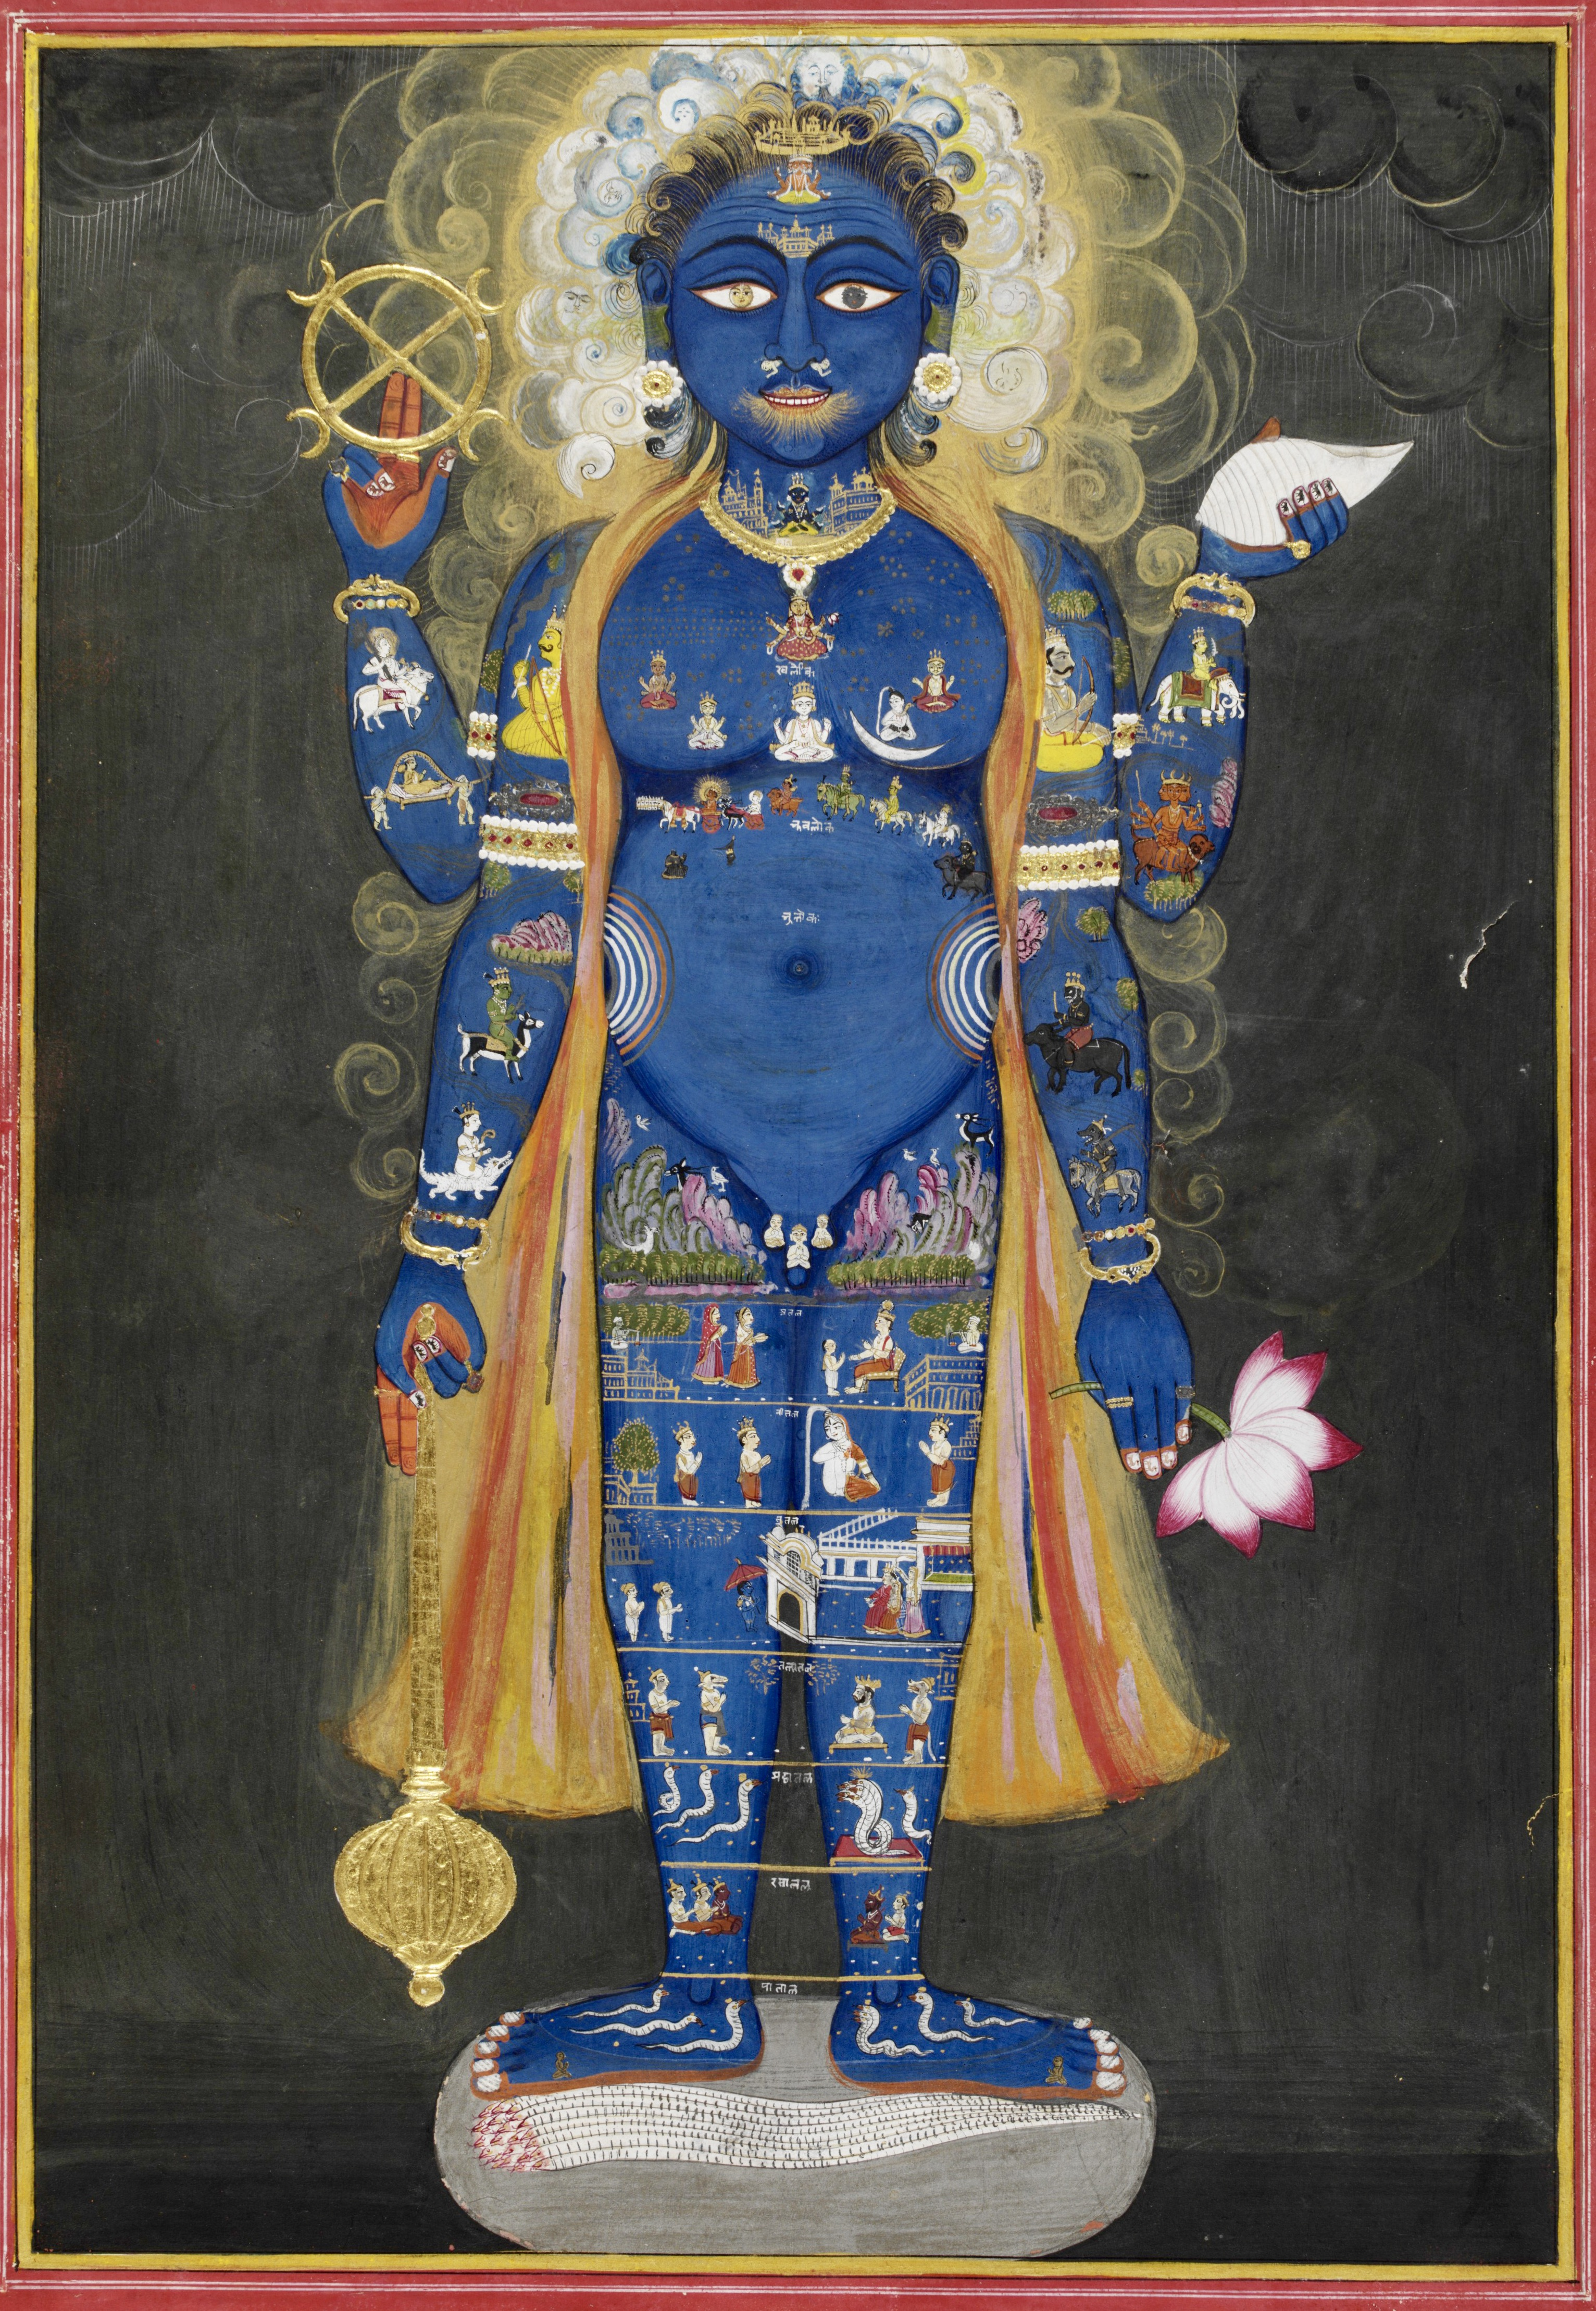
\includegraphics[width=1\textwidth]{pics/Vishnu_Vishvarupa_cropped.jpg}
	\caption{Viṣṇu Viśvarūpa, India, Rajasthan, Jaipur, ca. 1800–1820, Opaque watercolor and gold on paper, 38.5 × 28 cm, Victoria and Albert Museum, London, Given by Mrs. Gerald Clark.}
	\label{fig1}
      \end{figure}
\clearpage
  \begin{figure}[ht]
	\centering
  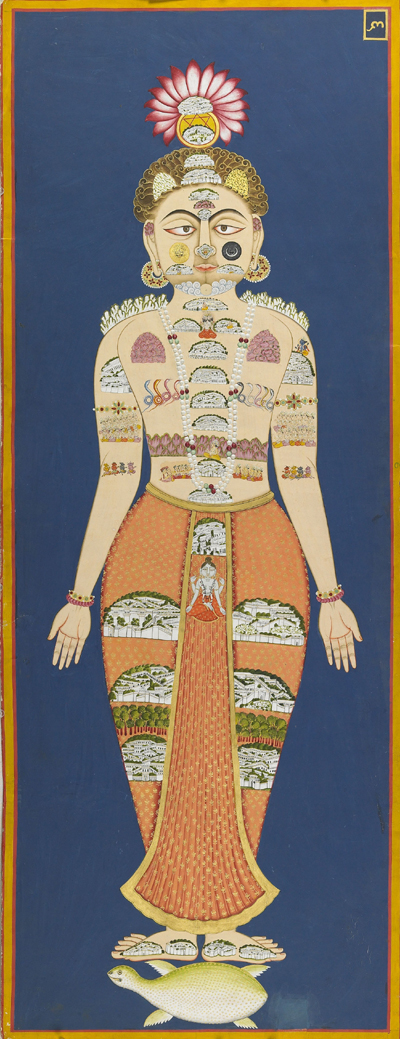
\includegraphics[width=0.5\textwidth]{pics/The_Equivalence_of_Self_and_Universe_(detail),_folio_6_from_the_Siddha_Siddhanta_Paddhati,_(Bulaki),_1824_(Samvat_1881);_122_x_46_cm._Mehrangarh_Museum_Trust..jpg}
	\caption{The Equivalence of Self and Universe (detail), folio 6 from the \textit{Siddhasiddhāntapaddhati} (Bulaki), India, Rajasthan, Jodhpur, 1824 (Samvat 1881), 122 x 46 cm, RJS 2378, Mehragarh Museum Trust.}
	\label{fig2}
      \end{figure}
      % \end{landscape}


\chapter{Bibliography}
 \label{sec:bibli}
   \clearpage
\newpage 
\thispagestyle{empty}
\quad  \addtocounter{page}{-1}

\printbibliography[heading=subbibintoc, title=Consulted Manuscripts, keyword=codex]

\printbibliography[heading=subbibintoc, title=Printed Editions, keyword=printsource]

\printbibliography[heading=subbibintoc, title=Secondary Literature, keyword=seclit]

\printbibliography[heading=subbibintoc, title=Online Sources, keyword=onlinesource]

\end{document}
